\chapter{Research}

I propose a framework to examine remixing in an online community of amateur creators. 
I approach this by first studying the design of the online community as a remixing system, and then analyzing what people do and how they react to what others do.
More specifically, I focus on the structural, functional and attitudinal characteristics of an online community's sociotechnical infrastructure and its participants activities.
This framework derives from and is examined through design interventions, three-years of participant observation data, case studies, interviews with community members, quantitative and network analysis of a large corpus of data that includes more than 700,000 registered accounts and a repository of more than 9 million comments and 1.6 million interactive media objects, 30\% of which are remixes.

\chapter{Structure of a Remixing System} 
I present an analysis of the sociotechnical architecture of the Scratch Online Community by examining its following structural attributes (Figure~\ref{fig:structure}):
1) granularity of the remixable components, 
2) modularity of the remixable components, 
3) decomposability of finished projects, 
4) attributability mechanisms, and 
5) openness to remix across systems.

I analyze these structural properties of the system using varied approaches including:
1) case studies that give a rich description of various scenarios that explain the influence of each attribute,
2) analyses of the data corpus to understand the frequency of the scenarios and the relationships among the structural attributes,
3) natural design experiments to study the effect of varying some structural dimensions.

\begin{figure} 
\centering
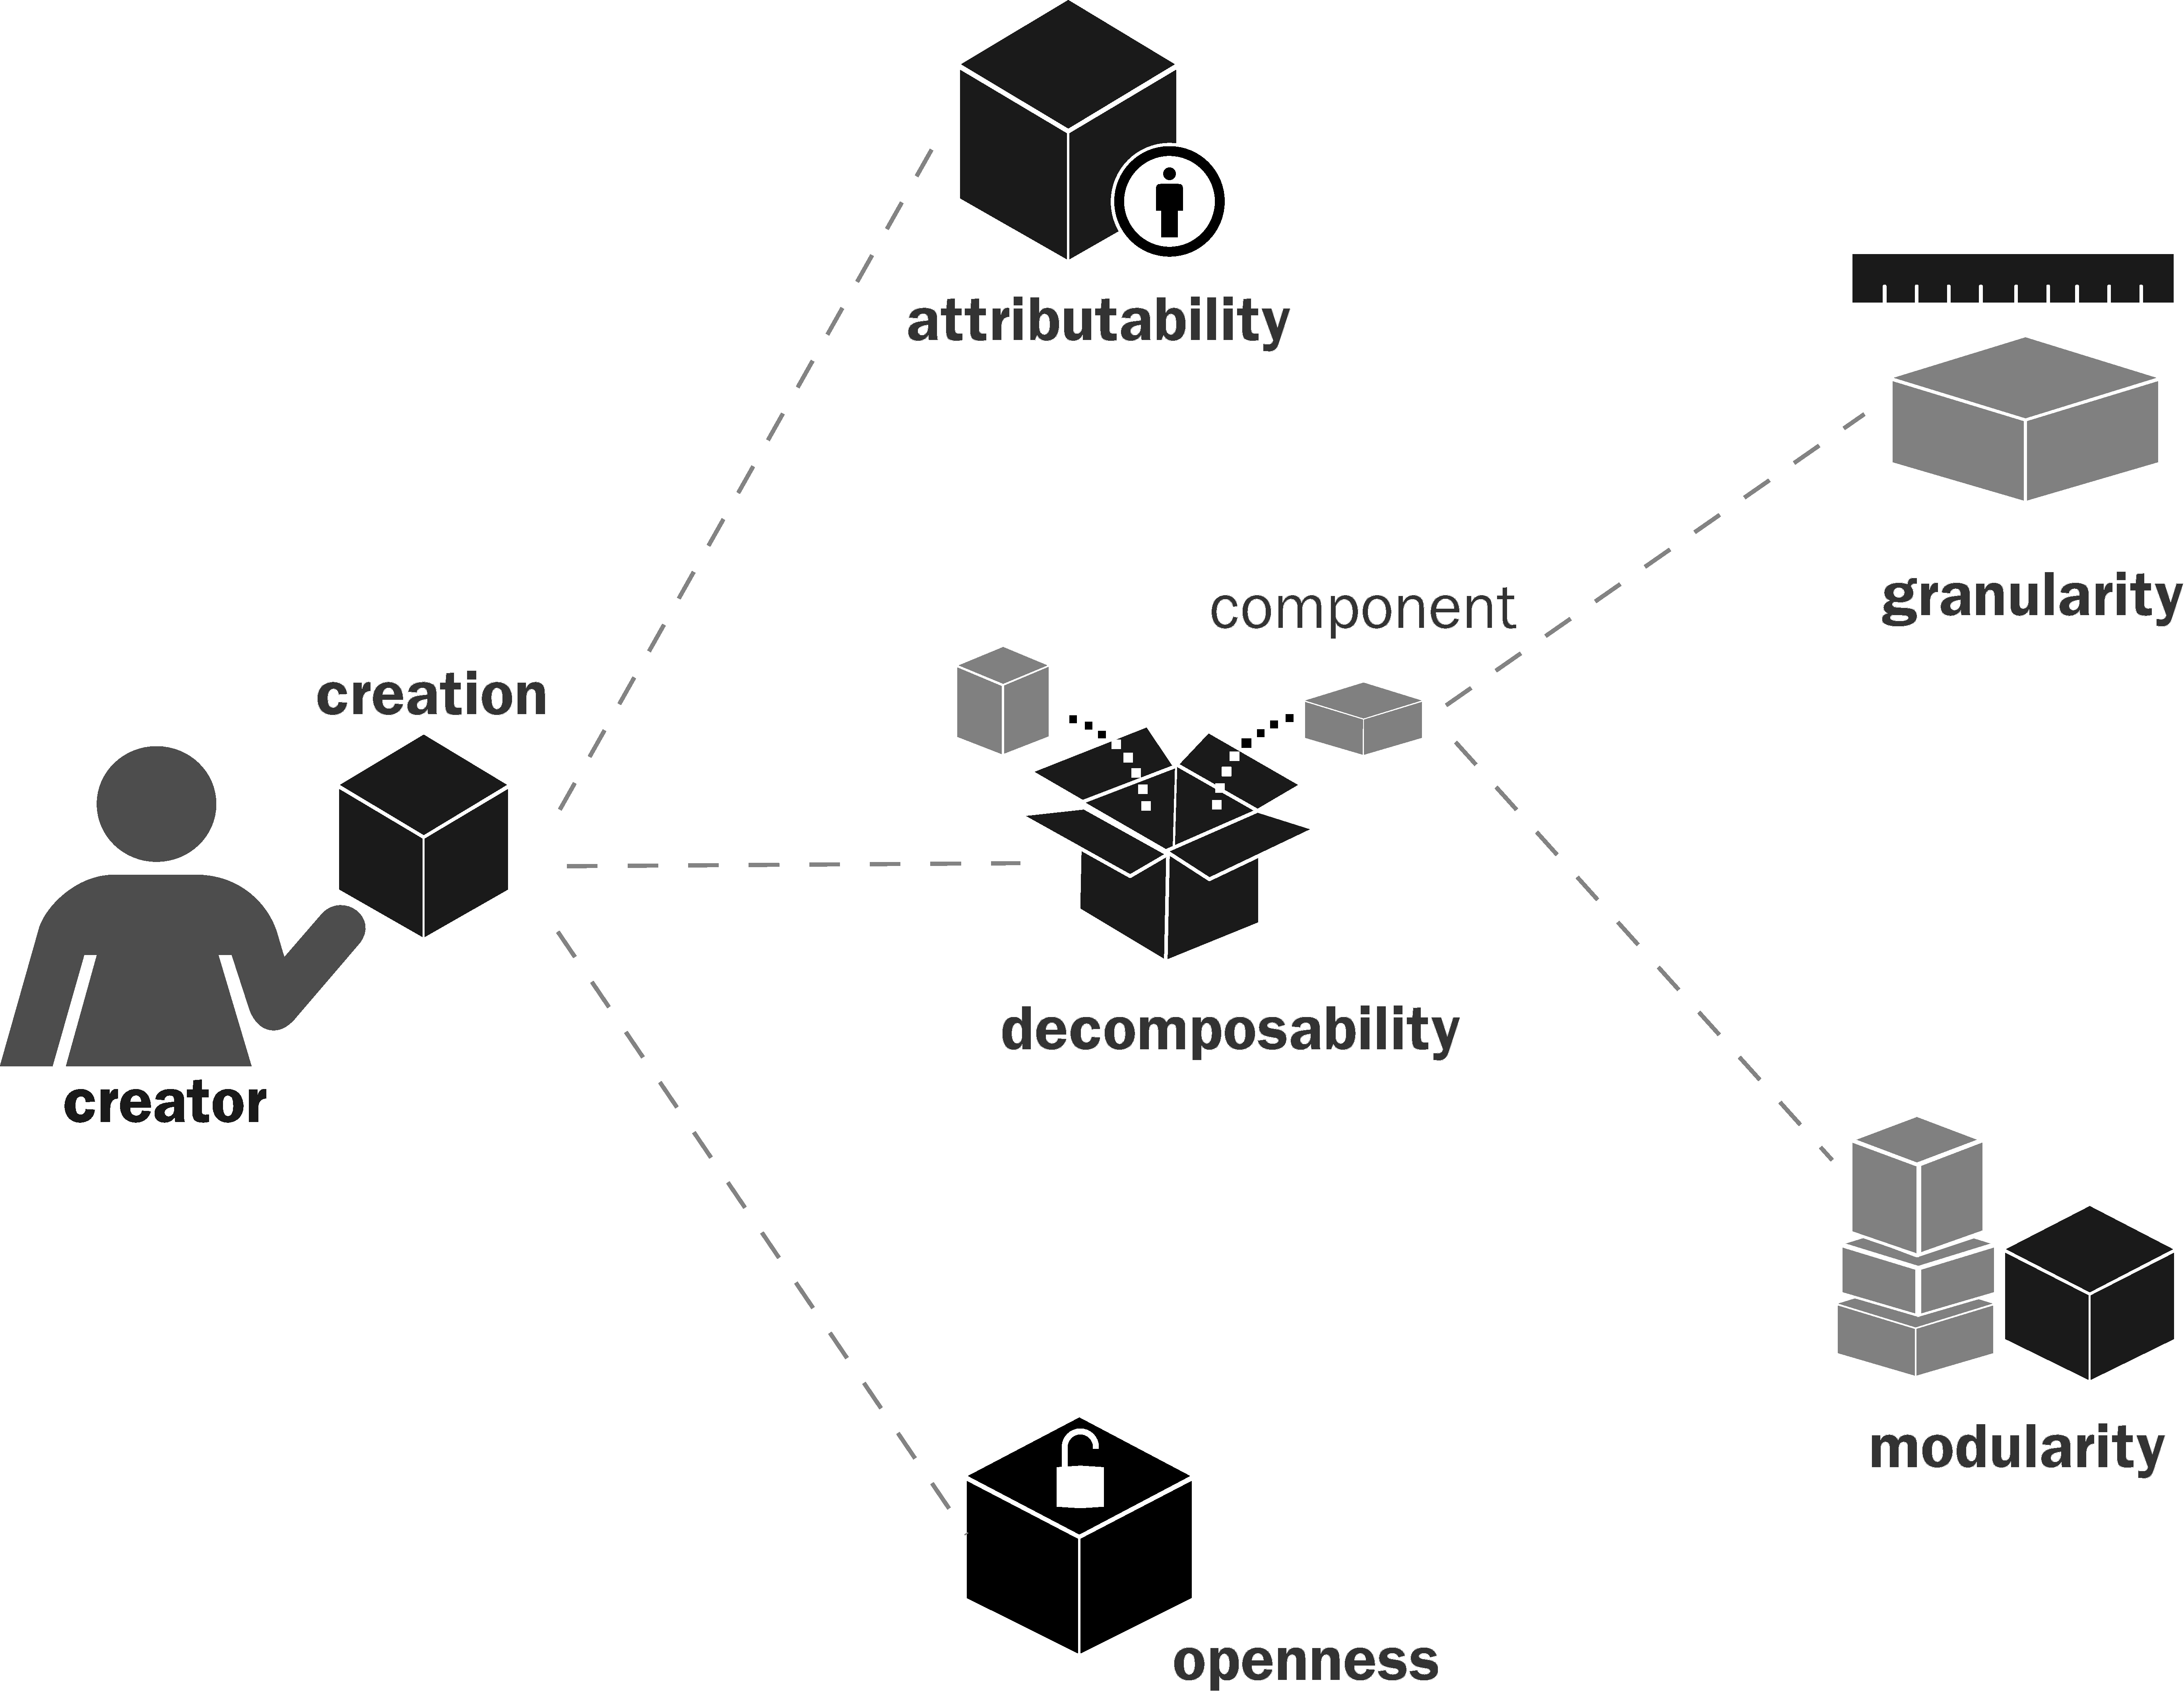
\includegraphics[width=3.25in]{figures/structure.pdf}
\caption{Structural dimensions of a remixing system (some icons taken from creativecommons.org, openclipart.org and thenounproject.com).}
\label{fig:structure}
\end{figure}

\section{Granularity}
Granularity is the size of project's modules \citep{benkler_coases_2002}. 
In Scratch, projects have several levels of granularity.
Projects are made of ``sprites'' such as characters in a game or elements in the user interface.
Each sprite can have ``scripts'' or stacks of programming blocks that control the sprite's behavior such as its position on the screen, its look, sound and interaction with other sprites and the user (by mouse, keyboard, or other sensors).
Each sprite also has one or more costumes or images that represent the various visual states of a sprite.
Sprites can also have sounds that are played programmatically; for example, a character in a game could make a sound each time it jumps.

\emph{Proposed Work.}
The Scratch Online Community, by default, only allows sharing at the coarsest degree of granularity: only projects can be shared. 
I analyze the implications of this design decision and the ways  people get around the limitations of the architecure.

I have anecdotal evidence that Scratch participants get around the granularity limitations by sharing full projects with the sole intention of sharing a single sprite, script, image or sound.
This need for finer granularity often stems from a desire to engage in sharing practices that the original design did not anticipate. 
% mres: not the clearest example of fine granularity % For example, in previous work \citep{nickerson_appropriation_2011}, we have documented the existence of ``coloring contests'' where someone creates a project inviting others to add color to an image and then several other people do so by remixing the original project.
I look at these practices in more detail to understand how a finer granularity mechanism would help support various types of creative and collaborative learning practices beyond the existing research that suggests that finer granularity is correlated with the number of people engaged in cooperative activities.

To analyze the effect of explicitly supporting finer degree of granularity through a natural experiment, I  analyze the adoption of ``Scratch Resources'' \footnote{Available at http://resources.scratchr.org}, a website created by members of the Scratch community to support sharing sprites, images and sounds. 
% TODO link to Von Hippel at al on user innovation

Some of my motivating questions are: 
How common is sharing and remixing across the various levels of granularity available (even if not explicitly supported)?
What are the types of participants and motivations for sharing finer grained components?
What role does granularity play in the likelihood of a project being remixed controlling for all other factors?
How do various levels of granularity affect the type and quality of remixes?
How do various levels of granularity support various levels of familiarity with Scratch -- are novices more likely to rely on coarser granularity when engaging in remixing as a scaffolding mechanism?

\section{Modularity}
\citet{benkler_coases_2002} defines modularity as the ``property of a project referring to the extent to which it can be broken down into smaller components, or modules, that can be independently and asynchronously produced before they are assembled into a whole.''
For this work, I separate two aspects of modularity:
1. The ease of \emph{integrating} such components into new creations or remixes.
2. The ease of \emph{decomposing} an existing project into smaller components, typically for remixing.
In this section I  analyze the term ``modularity'' by focusing on the first aspect.
In the next section, I focus on the second aspect under the term ``decomposability''.

\emph{Proposed Work.}
Some components or projects can be more easily integrated into new projects. 
One of the questions I am interested in exploring is what makes some components more modular than others.

For example, an image generated programmatically might be harder to integrate than one in bitmap format. 
A module that represents a cultural icon, such as Mario\footnote{Mario is a character in a popular video game called Mario Bros. from Nintendo Inc.}, is perhaps easier to integrate into other projects than an image of a less well-known character.
However, there are situations when new subcultural icons emerge within the Scratch community.
For example, a community member from New Zealand created a character called Maki-Tak. 
Maki-Tak became so popular in the community that other people started to create projects that included Maki-Tak itself of  that character or other characters inspired by it, often called Takis.
% Other examples: Mr Happy Man
Situations exist where some components are remixed despite their internal complexity, which might indicate that these could be built in a way that their internal complexity is hidden and remixing them is easy. 
For example there is a sprite created by an advanced Scratch user that represented a physics simulation of a string. 
This project was later remixed in a project where it represented a necklace.

I  operationalize the assessment of modularity by measuring its adoption through a number of remixes.
The assumption is that more modular components are remixed more.
I examine this in two types of components: the sample sprites, images and sounds that come with Scratch, and the ones that members of the community have created.
% Sample components are those that come preinstalled with Scratch. For example, sample images, sounds, sprites and occasionally projects.
% Community-generated are those created by end-users.
% The following paragraphs are commented out because mres mentioned that jetpack girl is not clear, plus I should make this research section shorter
%For example, ``jetpack girl'' is a sample sprite consisting of five costumes and  sounds for a flying character that can be controlled with the keyboard.
%The code of the sprite comes with an invitation to remix: ``Import me into your own project'' and an explanation on how to use it ``arrow keys make me fly''.
%These sample components are not only sprites, there are also hundreds of images and sounds that come with Scratch such as photographs of people, animals, things, and so on.
%Besides these sample components, there are thousands of components created by community members that are remixed and can be found in places like Scratch Resources and Scratch projects that explicitly state that they include sprites, images and sounds for others to reuse.

The type of questions I will to answer are:
1. What technical or cultural attributes are linked with component modularity? 
2. Are modular components used more often by newcomers, and do they provide scaffolding in their learning of Scratch programming?
3. Are community-generated components more often created by advanced users?

\section{Decomposability}
Building on the concept of modularity examined before, in this section I examine decomposability as the ease of decomposing a compiled project.
Decomposability is the ease of breaking something apart for remixing.
Therefore decomposability depends on the internal complexity of a project, which in itself depends on the expertise of the person attempting to decompose the project.
For example, one can argue that images in Flickr.com are harder to decompose than those in OpenClipart.org, which provides the source vectors, or Aviary.com which provides the bitmap images that were used to create an image.
The same happens with software applications that provide the source code in contrast with those that only provide the final compiled executable.
But even if the source code is provided, there are some cases where projects are ``impenetrable'' because of their complexity or a mismatch between the expertise of the person trying to decompose a project and the complexity of the project. 
For example, for a novice programmer having access to the source code of the Linux kernel might not allow for easy decomposability.

In Scratch, all the sources of a project are provided so the decomposability of a project depends, among other things, more on how interconnected its various components are. 
For example, sometimes sprites ``broadcast'' messages back and forth making their decomposability much harder than those that are self-contained.
Also some creators add instructions to their projects explaining how they can be broken apart, while others obfuscate their code to prevent remixing.

\emph{Proposed Work.}
I first do a manual analysis of a sample of projects to observe patterns of decomposability. 
Using the findings of this analysis I devise mechanisms to automate the evaluation of decomposability. 
For example, a decomposability metric could depend on the use of particular blocks (the ``broadcast'' block could reduce its ranking, while comments in the code would increase it), explicit obfuscation or matching between the typical expertise level of community members and the expertise required to understand a project.

I also look at remixes to analyze how different they are from their original project. 
The assumption would be that ``impenetrable'' projects would be correlated with no remixing or to superficial remixes, such as slight changes in the images, while highly decomposable projects are associated with significant differences between the remix and the original.

I also analyze the practices of code obfuscation and the strategies people use to discourage decomposability of their projects.

\section{Attributability}
Creators often want to get credit for their work. 
For example, the Creative Commons license originally had attribution as one of the options of their licenses, but after analyzing several years of usage of the licenses they found that few people waived the attribution clause. 
This led them to include attribution by default in all their licenses (and create a separate license for completely public domain works) \citep{brown_announcing_2004}.
To further our understanding of attribution when designing a remixing system it is important to know the role attribution plays in supporting cooperative behavior among members of a remixing online community.

In Scratch, we have run some design experiments playing with attribution. 
For example, we found evidence that suggests that about 20\% of creators object to seeing their projects remixed \citep{hill_responses_2010}.
We also have anecdotal evidence that people, who objected to remixing of their project, referred to a lack of credit as one of the problems.
To address this, I added a mechanism that would automatically give credit to the creator of the original project whenever a remix was uploaded (for example, ``Shared by John, based on Mary's project'').
Using that design intervention as a natural experiment, we found evidence that suggests people not only want to get credit but that they prefer the credit given by another person over the automatic attribution given by the system \cite{monroy-hernandez_computers_2011}. 

\emph{Proposed Work.}
I  extend this work with additional experiments.
For example, one of the common complaints against remixing is that the textual description of projects often gets copied from an original project onto its remixes.
This often gives the wrong impression that those notes were by the remixer rather than by the original creator.
I  add a mechanism to show a distinction between the notes by the originator and those added by the remixer.
These additional notes come with a mechanism to encourage remixers to explain how the original project was changed.
This will serve as a natural experiment to test the additional value of not only giving binary representation of attribution but also give a qualifier explanation to the connection between a remix and the original project.

% TODO: Other experiments: 
% - Creator endorsed attribution.
% - Diff

\section{Openness}
In this section I focus on analyzing a system's openness from the perspective of its norms and interactions with other systems.
The Scratch Online Community allows any of its members to download and remix any project, in that sense Scratch is more open than similar websites such as Kongregate.com or Newgrounds.com, which do not provide either the license, the environment, nor the technical features to freely open its content. 
The ethos of openness is present in Scratch through its terms of use, the license used by all projects shared, and the community moderation styled enforced by administrators.
However, this openness is not always understood or embraced by its members.
Also this openness is not always compatible with other systems.
For example, there are a some members of the community, who even after discussions with the administrators of the site, do not see enough value of openly sharing their work and decide to stop using the website. 
Additionally, there are other members of the community who encounter conflicts when remixing content from other online spaces that are not compatible with Scratch's openness. 
These conflicts often involve art-sharing websites like DeviantArt.com, from where Scratch creators sometimes get images for their projects.

\emph{Proposed Work.}
I  investigate the ways young people in Scratch embrace, understand and reject the way openness is interpreted in Scratch.
I try to examine whether young people see a value in openness and how a system is or is not able to surface these values through sociotechnical design.
I present a set of case studies that show the range of ways people embrace and reject openness and how the social and technical design of the website influence them. 



\chapter{Functional Role of Remixing}

The previous section helped describe the structural properties of the Scratch Online Community as a remixing system.
This section is intended to examine what people do.
In particular, the goal is to understand what are the various roles that remixing plays and how it is part of collaborative and creative practices.

\begin{figure}
\centering
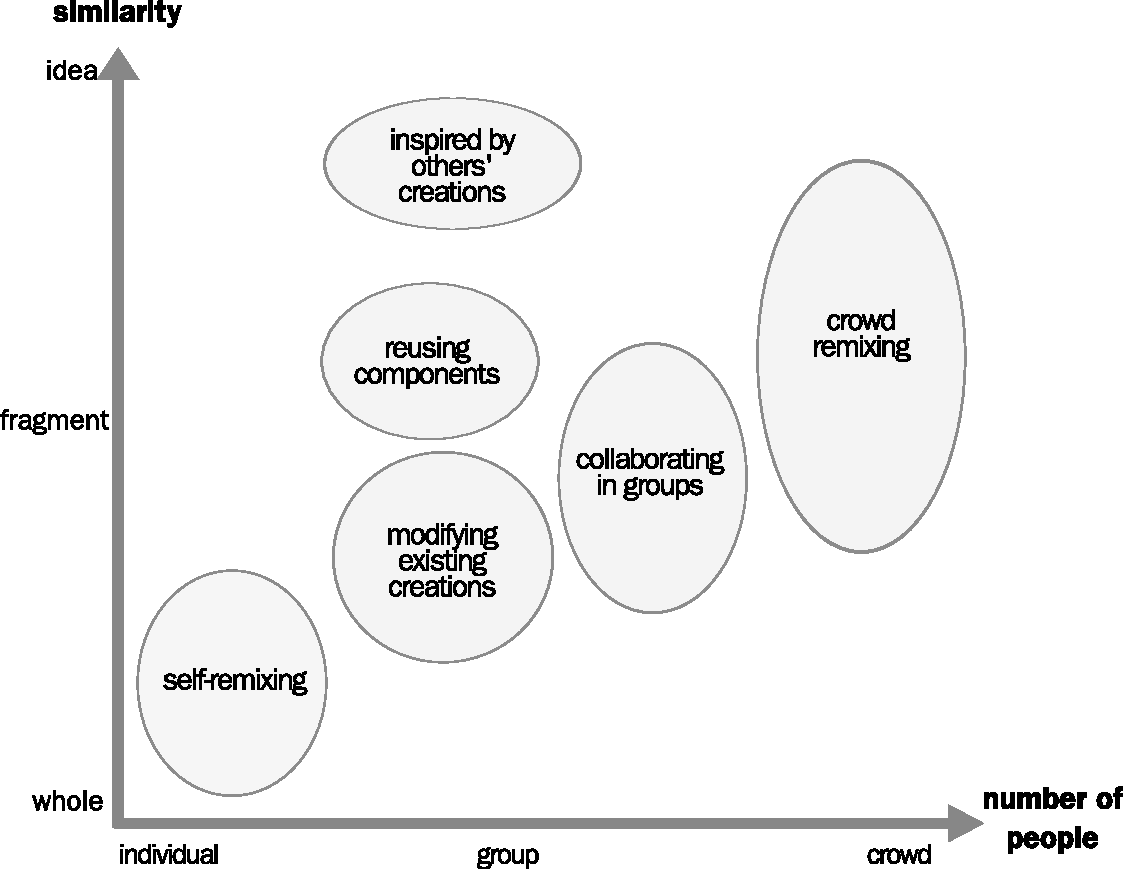
\includegraphics[width=3.25in]{figures/function.pdf}
\caption{Functional roles of remixing in the social and product-focus dimensions}
\label{fig:function}
\end{figure}

Remixing represents many activities in Scratch.
For example, people occasionally remix to fix software bugs on someone's project; in other cases people want to add to an existing project to customize it or make it more personal; in others, people want to start a trend or ``meme'' so they create a ``template'' project just so others remix it, add to it and pass it on.

To map these varied types of remixing, based on previous analysis of other remixing online communities \citep{seneviratne_remix_2010}, I focus on two dimensions:
\begin{enumerate}
\item{Similarity}. This indicates how different a remix is from the original work on which it is based. 
Remixes can range from merely being inspired by someone's idea, to tweaking someone's project, to making an exact copy.
This is an important aspect of remixing because it gets at the core of some of the tensions around remixing, and it also helps us understand the degree of interaction and creative output between a remix and its antecedent project.
\item{Number of people}. This indicates the number people involved or intended to be involved in the remix.
Remixes can range from a single author (for example, a creator remixing herself as a form of version control), to a small group of people (for example, a team collaborating in making projects), to a crowd (for example, a large group of people participating in a remix chain).
The number of people involved is a useful dimension because it helps us identify the distinct roles remixing plays in Scratch.
\end{enumerate}

Using these two dimensions, one can identify a set of remixing categories (Figure~\ref{fig:function}) useful for the analysis of the functional roles of remixing in Scratch.
Broadly speaking, the types of remixing I  use to guide my analyses are the following:

\section{Incremental Remixing}
This type of remixing often involves downloading someone's project to customize it or to fix a bug. 
For example, replacing the costumes of a sprite in a game for a different one. 
This form of remixing often occurs when people make small modifications to the sample projects that come preinstalled with Scratch.
Also anecdotal evidence suggests that this form of remixing tends to be a useful way for newcomers to get started with Scratch,  modifying an existing project instead of creating a completely new project.
This type of remixing sometimes leads to controversy when the changes are subtle or nonexistent.
Project creators sometimes argue that types of remixing in which the changes are minimal should not be allowed.

\section{Component Remixing}
Remixing also occurs when people use pieces of others' projects to produce something new, rather than building on top of existing work.   
In these cases, often one cannot quickly tell in what way the remix and the original are related.
This type of remixing typically involves some sample sprites that come preinstalled with Scratch, such as the ``jetpack girl'' example mentioned above or some templates, images or sounds that members of the community created for others to reuse.


\section{Group Remixing}
Remixing is also used by groups or ``collabs'', as they are often referred to by Scratch members, to work collaboratively by remixing one another's work almost as a form of version control \citep{tichy_rcs_1985}.
For example, we found in that one of the ``collabs'' we analyzed, one member of the group would start by creating a first version of the project they had decided to make while others would work on varied parts such as the images, sounds or the engine of a game \citep{aragon_tale_2009}.
In that particular ``collab'' there were, on average, seventeen remixes before officially releasing a project.
In this case, remixing is part of an explicit collaborative activity.


\section{Crowd Remixing}
The home page of the Scratch website has a section called ``What the Community is Remixing''  that features the three top remixed projects in the past two weeks.
Although these projects could represent any type of remixing, they are typically projects that consist of a compelling template that encourages people to add something small to it and pass it on to someone else, like a chain.
For example, one of those projects titled ``Add yourself to the party'' shows a character dancing on a colorful dance floor by itself.
The creator leaves a note in the description of the project inviting people to download the project and add a sprite representing their avatar or profile picture.
Other examples are ``Remix if you care about animal rights'', representing a type of crowd remixing with a social cause, and ``Coloring contest'', representing popular genre among more artistic-inclined community members that consists of downloading a still image (often with music playing in the background), coloring it and submitting it to a contest for the best-colored image.
Although typically the intention of the creator of this type of project is to create a chain, often the structure of the remix network looks more like a star because of people not following the rules or not checking where the last element of the chain is.
These types of remixes are often incremental like the category described above, but the relationship between the creator and its intended audience is significantly different. 
Crowd remixing explicitly invites people to remix en masse following a specific template. 
The purpose of the creation is not the creation itself but the collection of many remixes created by many individuals.
Evidence suggests that this type of crowd remixing emerged after the top remixed projects section was added to the website, but more research is needed to understand these phenomena.

\section{Inspirational Remixing}
On the far end of the similarity spectrum are projects that are inspired by other projects that do not use any particular component of the original work.
These projects are often trying to replicate popular software, video games or even genres that have emerged in the community.
For example, some people create remixes of the Microsoft Windows operating system, or the iPhone, or operating systems that other members of the community have created such as SynOS, a popular Scratch-based pseudo-operating system created by a teenage member of the community.
Other examples of inspirational remixes are the ``fan art'' projects created after popular characters created by other members of the Scratch community such as ``Maki-Tak'', a lizard that dances and sings in animations created by a teenage girl,  or  ``Mr. Happy Man'', a grumpy character invented by a teenage boy.
This type of inspirational remixing is a lot harder to identify automatically because the original and the remix do not share any bytes but their names, descriptions and log data might help. 

\section{Self-remixing}
%  TODO: Check this number.
About 13\% of remixes are projects created based on the same person's projects.
This is typically used as some form of version control.
For example, sometimes children create a Scratch project at school, upload it to the website, download it at home, continue working on it, then re-upload it to the website under a name like ``My video game v2''.
When this happens, the website identifies them as remixes and links them back to their previous version.
A few people, mainly popular Scratch creators who care about the projects displayed on their profile page, have two accounts: one for testing and one for sharing final version of their projects.
For example, there is an adult member of the community who has two usernames: ``Paddle2See'' and ``Paddle2SeeTest''.
As the name implies, one is often used for sharing drafts or work in progress.
 
\section{Proposed work}
In this section of my dissertation I  describe the way people engage in remixing on the Scratch Online Community. 
In particular, I  answer questions such as:
1. Are the types of remixing described above representative for Scratch and generalizable for other online remixing communities? 
For this, I  connect with other researchers investigating other online communities, especially ccMixter.org.
2. What kind of people engage in each type of remixing? For example, do novices engage in incremental and crowd remixing more often than component remixing? Are the originators of crowd remixing longtime members of the community and how do they manage to get more people to remix their work?
3. In what way does each type of remixing help scaffold Scratch participation? For example, are some types of remixing better at learning the technical aspects of Scratch while others are more helpful in learning how to collaborate and socialize online? Are people who engage in remixing initially more likely to stay active on the community and in what ways?
4. How have these types of remixing evolved over the course of three years?
Are the social networks created through various types of remixing different in their structure and quality?
5. How do the projects in each type of remixing differ technically and in content? For example, in what ways might some types be more complex than others?
The distinctions amongst the types are subjective at this point, and part of the work I  do is to clearly identify the boundaries among categories.



\chapter{Attitudes Toward Remixing}

I investigate remixers' and originators' attitudes toward remixing. In particular, I analyze how participants perceive remixing and how they do or do not cooperate by letting or encouraging others to reuse their work.
This analysis is driven by an interest in understanding how the system design may influence these attitudes. 
I analyze these issues from the perspective of people whose projects are remixed as well as from those creating the remixes.
 
Previous work studying people's attitudes toward remixing in the Scratch Online Community \citep{hill_responses_2010, monroy-hernandez_computers_2011} found evidence that people are as likely to react negatively as they are to react positively when someone remixes their work. 
Additionally, we have found originators are more likely to respond negatively when their projects are more complex.
Broadly speaking, people whose projects are remixed react either by being indifferent to it, accepting it, conditionally accepting it (for example, specific rules or norms have to be followed), or by explicitly opposing to it (for example, posting a negative reaction comment like ``you stole my project!'').
Similarly, remixers go about remixing by either being oblivious of the norms (for example, giving credit or asking for permission has emerged as a norm in the  community), or cautiously doing it by asking for permission first, or even being confrontational and using remixing as a form of ``trolling'' \citep{donath_identity_1998}.

In this work, I analyze people's attitudes toward remixing in the Scratch Online Community through case studies and experiments.
Additionally, I expect these metrics of people's responses and attitudes will serve to understand the health of the community and to motivate further design interventions.
In particular, I propose two studies for studying Scratch participant's attitudes toward remixing that complement the two recently published articles \citep{monroy-hernandez_computers_2011,hill_responses_2010}.

% FROM CHI

In this paper, we employ a mixed methods approach that combines
qualitative and quantitative analyses to explore users' reactions to
attribution and its absence in a large remixing community. First, we
introduce our empirical setting; using qualitative data from users
forums and comments, we present a rich description of remixing and
evidence to support our core proposition that credit plays a central
role in remixing in our environment. Second, we contextualize and
describe a technological intervention in our setting, responding
directly to several user suggestions, that automated the attribution
of creators of antecedent projects when content was remixed. Third, we
present a tentative quantitative analysis of the effect of this
intervention along with a parallel analysis of the practice of manual
credit-giving. We find that credit-giving, done manually, is
associated with more positive reactions but that automatic attribution
by the system is not associated with a similar effect. Fourth, we
present analysis of a set of in-depth interviews with twelve users
which helps confirm, and add nuance and depth to, our quantitative
findings.

Our results suggest that young users see an important, if currently
under-appreciated and under-theorized, difference between
\emph{credit} and \emph{attribution}. Credit represents more than a
public reference to an ``upstream'' user's contributions. Coming from
another human, credit can involve an explicit acknowledgment, an
expression of gratitude, and an expression of deference, in a way that
simple attribution can not. Our results suggest that identical
attribution information means something very different to users when
it comes from a computer, and when it comes from a human -- and that
users often feel that acknowledgment is worth much less when it comes
from a system. We conclude that designers should create affordances
that make it easier for users to credit each other, rather than to
merely pursue automated means of acknowledgment.

Our study offers two distinct contributions for social scientists and
for technology designers.  The first is an improved understanding of
the way that attribution and credit work in user-generated content
communities. The second is a broader contribution to the literature on
design that suggests an important limitation to technologists' ability to
support community norms and a suggestion for how designers might
create affordances. Functionality that allows users to
express information that a system might otherwise show automatically
may play an important role in successful design for social media
environments.


% NOTES The overarching questions are: How do young people respond to remixing? How are these attitudes represented in the community? When do they embrace remixing and when do they reject it?  I have and will analyze young people’s attitudes based on their words (interviews) comments, reports (flags) and strategies for deterring (obfuscation, pseudo-licenses, Vigilantism) or supporting remixing (commenting, scaffolding, framework approach, creation of narratives).
% Crowding out remixing by featuring
% Evolution of reactions as design changes

%TODO: the following studies are from our ICWSM paper. Need more paraphrasing.
%TODO: the following studies are from our ICWSM paper. Need more paraphrasing.
%TODO: FIX REFERENCES
The analysis on people's responses to remixing on Scratch consisted of three studies:

\section{Study 1: How do people respond to remixing?}

In Study 1, we assess Scratch users' reactions to having their projects
remixed. To do so, we created an algorithm to
identify all original-remix pairs in the first
13 months of the Scratch community. These pairs were made up of all
projects based on another project and its corresponding antecedent.  We
subsequently coded all comments left by the author of the original
project (i.e., the {\em originator}) on each remixed project.

Our algorithm identified projects based on metadata embedded in projects. As a result, we
would not count projects that were conceptually copied by a user who had
seen another's work but who did not actually copy code, graphics or
sounds.  Additionally, as there were over 100,000 projects, we could not
feasibly watch and interact with each project and determine whether the
original projects were actually ``original'' or whether ideas were taken
from a source outside Scratch (e.g., a user may have created a Pacman
clone).

Broadly speaking, people whose projects are remixed react either by being indifferent to it, accepting it, conditionally accepting it (for example, specific rules or norms have to be followed), or by explicitly opposing to it (for example, posting a negative reaction comment like ``you stole my project!'').
Similarly, remixers go about remixing by either being oblivious of the norms (for example, giving credit or asking for permission has emerged as a norm in the  community), or cautiously doing it by asking for permission first, or even being confrontational and using remixing as a form of ``trolling'' \citep{donath_identity_1998}.

% NOTE: originally removed due to space limitations in ICWSM paper
If a user created a Pacman clone and it was then modified or
improved by another Scratch user, the second user would be considered a
 ``remixer'' in our data set while the first would not.

\subsection{Procedure}

We applied our algorithm to all 136,929 projects created and posted on the
Scratch website between the community launch date in March 2007 and
April 2008 to identify all derivative projects;
a total of 11,861 projects were deemed to be based on other projects.
The comments left by originators on the first
3,555 projects were coded by two independent coders who were asked to
code all projects into the following categories: {\em no comment}
(projects in which the originator did not leave any comments on the
remixer's project), {\em positive} (projects in which the originator
left positive comments, e.g., ``Love what you did with my code! Great
idea!''), {\em hinting plagiarism} (projects in which the originator
implied that the remixer had copied but did not state this explicitly,
e.g., ``I mostly pretty much made this whole entire game''), {\em
plagiarism} (projects in which the the originator directly accused the
remixer of copying, e.g., ``Hello mr plagiarist”, ``Copy-cat!''), {\em
negative} (projects with negative comments that were not necessarily
related to copying, e.g., ``Alright you crap eating thumb sucking
baby''), and {\em none of the above} (projects with comments that were
not positive, negative, or relevant to plagiarism, e.g., ``is this
jarred'' or ``b for peanut butter jelly time!'').

The first and last categories were mutually exclusive from all others.
The other categories were potentially overlapping (an originator could
say, ``you copied me but I like your addition of the flowers'' and
therefore count as {\em positive} comments and {\em plagiarism}), with
the exception of {\em hinting plagiarism} and {\em plagiarism} which were mutually exclusive of each other. The coders were found to be reliable (absolute
agreement by category: {\em no comment}=100\%; of those that did include
a comment, coders agreed on the presence or absence of the following
categories at the following rates (absolute agreement): {\em
positive}=87\%, {\em hinting plagiarism}=81\%, {\em plagiarism}=89\%,
{\em negative}=93\%, {\em none of the above}=89\%). Therefore the
remaining comments (n=8,306) were split between the two coders, with
each coding approximately half of the remaining projects. For the few
projects that the coders disagreed on in the initial third of the
projects, they met and came to an agreement on the coding.


\subsection{Results}

Out of the 11,861 projects that were categorized by the algorithm as remixes,
we were able to determine that 3,742 (31.5\%) of the original creators
clicked on and saw the remixed versions of their projects. Of
those originators who saw the projects, 2,156 (58\%) did not leave a
comment.  Of those who saw the projects and commented, 261 (7\%) accused
the remixer of plagiarism, 566 (15\%) hinted at plagiarism concerns, 797
(21\%) left positive comments, 260 (7\%) left negative comments, and 237
(6\%) left comments that did not fit into these categories or were
uninterpretable.

\subsection{Discussion}

The results from Study 1 indicate that users on the Scratch online
community have a wide range of responses to remixing. People who responded were just
as likely to leave positive comments (21\%) as they were to leave a
direct or indirect complaint of plagiarism (22\%). These results
however, leave open the question of why such a wide range of comments
were left by originators. Several potential answers to these questions
are explored in Studies 2 and 3.

\subsection{Implications for design}

The Scratch online community was designed explicitly as a platform for
sharing and remixing media. Despite the fact the Scratch
infrastructure provided the technical facilities to remix content
easily, a set of explicit norms and licenses communicated to
users through links to a child-friendly version of the
pro-remixing license on every project, and continuous proselytizing of
remixing by the administrators of the site, many users reacted
negatively to remixes and expressed a sentiment that remixers had
plagiarized their work.

Creative Commons has described its work, both through the creation of
licenses permitting remixing and through the creation of technological
systems built around RDF (Resource Description Framework) metadata, as
means of reducing permission-asking \cite{lessig_keynote_2004}. Like
Scratch, many social media and remixing communities use CC's legal and
technological systems.  To the degree that our results generalize, our
findings suggest that the technical and normative permission to create
remixes may be insufficient to supporting positive reactions to remixing
in a social media remixing community.

% NOTES The overarching questions are: How do young people respond to remixing? How are these attitudes represented in the community? When do they embrace remixing and when do they reject it?  I have and will analyze young people’s attitudes based on their words (interviews) comments, reports (flags) and strategies for deterring (obfuscation, pseudo-licenses, Vigilantism) or supporting remixing (commenting, scaffolding, framework approach, creation of narratives).
% Crowding out remixing by featuring
% Evolution of reactions as design changes

\section{Study 2: When do originators accuse\\ remixers of plagiarism?}

% TODO: FIX TABLE. DOESNT COMPILE.
% latex table generated in R 2.10.1 by xtable 1.5-6 package
% Thu Mar 11 15:01:16 2010
%\begin{table*}[ht]
%\begin{center}
%
%\begin{tabular}{rrrrrrrrrr}
%  \hline
% & Mean & SD & 1 & 2 & 3 & 4 & 5 & 6 & 7 \\ 
%  \hline
%1. ACCUSE.PLAG & 0.13 & 0.34 &  &  &  &  &  &  &  \\ 
%  2. SPRITES & 9.05 & 12.24 & 0.08 &  &  &  &  &  &  \\ 
%  3. ORIG.REMIX & 0.05 & 0.21 & -0.01 & 0.00 &  &  &  &  &  \\ 
%  4. HAS.REMIXED & 0.79 & 0.41 & -0.01 & -0.07 & 0.11 &  &  &  &  \\ 
%  5. FEMALE & 0.25 & 0.43 & -0.06 & -0.11 & 0.04 & 0.11 &  &  &  \\ 
%  6. WEEKS & 35.15 & 14.49 & 0.01 & -0.03 & 0.08 & 0.15 & 0.15 &  &  \\ 
%  7. AGE & 17.08 & 10.15 & -0.07 & 0.08 & 0.01 & -0.08 & -0.20 & -0.16 &  \\ 
%  8. REMIXER.AGE & 15.01 & 9.58 & -0.05 & 0.01 & 0.06 & -0.09 & -0.05 & -0.05 & 0.11 \\ 
%   \hline
%\end{tabular}
%
%\caption{Means, standard deviations, and correlations between variables
%used in the logistic regression analysis in Study 2. The sample includes
%all remixed projects that had been clicked on and viewed by the
%originators. ($n$=3742)}
%
%%\label{tab:cor}
%
%\end{center}
%\end{table*}

There are several explanations for the wide variety of reactions to
remixing shown in Study 1. In Study 2, we use the results of Study 1 to
construct a variable measuring whether originators have accused a
remixer of plagiarism.  We use this construct as the dependent
variable in a series of fitted logistic regression models to provide
initial tests of support for several explanations of why originators may
accuse remixers of their work of plagiarism using additional data on projects
and their creators.

One difference between Scratch and some other online peer-production
communities is that many Scratch projects are constructed at enormous
individual effort. On Scratch, users share full-fledged games or
animations with code, artwork and sound.
This is in contrast to many peer production communities, like
Wikipedia, where users usually contribute smaller portions of articles or
small fixes. One explanation for the high number of
complaints on Scratch may be that Scratch users develop a stronger sense
of ownership because of the large amount of individual time and effort
creators invest in their projects. This sense of ownership may set users
up to be more protective of their work and more likely to accuse
remixers of plagiarism.  This explanation leads us to our first
hypothesis (H2-1): {\em Originators of larger or more complicated
contributions will be more likely to accuse remixers of their projects
of plagiarism.}

In many peer production communities, like Wikipedia, the vast majority
of contributions are to existing products and work is primarily
cumulative in nature. In our sample of 11,861 remixes from the first year of Scratch's activity, the large majority of remixes (11,493 or 97\%) were based on
projects that were created {\em de novo} while the remaining were second
generation remixes. If users feel more protective of projects that are
entirely the product of their own work, an explanation for the high
number of complaints in Scratch is that because such a large number of
Scratch projects are created {\em de novo}, Scratch users are more
likely to feel plagiarized when their work is remixed. This leads to our
second hypothesis (H2-2): {\em Originators will be less likely to accuse
remixers of their projects of plagiarism when the remixed project is
itself a remix.}

A final explanation extends this reasoning from the project level to the
individual. Perhaps the process of creating remixes encourages
originators to be empathetic toward remixers and to integrate these
users into a ``remixing culture'' where copied or slightly modified
projects are not seen as plagiarism but rather as positive
contributions. In our sample, most authors of remixed projects were
active contributors who have, at some point in time, created their own
remixes.  Indeed, only 26\% of users in our sample (n=3,085) have never
shared a remix. It is possible that a large portion of charges of
plagiarism come from users who have not been integrated into Scratch's
``remix culture'' and are opposed to remixing in general.  This
explanation leads to to the formation of our third hypothesis
(H2-3): {\em Originators will be less likely to accuse remixers of their
projects of plagiarism if they have shared at least one remix
themselves.}

Of course, other factors are likely to have an important impact on
responses to remixing in Scratch that we feel it is necessary to control
for.  For example, charges of plagiarism may be due, in part, to the
large number of projects created by males in our sample (only 25\% of
originators were female) who may be more likely to accuse others of
plagiarism.  Additionally, the proportion of projects that are remixes
has increased over the life of our study. This suggests that attitudes
toward remixing may have changed over time with the potential for a
change in plagiarism accusation rates.  Finally, younger originators may
be more likely to accuse remixers of plagiarism either because they do
not understand that they are giving permission to others to remix by
sharing their work, because younger users are more likely to react
negatively in general, or for any number of other factors that correlate
with age.  As a result, we will control for gender, the time period when
projects were shared, and age, when testing the above hypotheses.

\subsection{Procedure}

To explore these issues, we used a sample consisting of the 3,742
remixed projects that had been clicked on and viewed by the originators,
as described in Study 1.  Viewing a project is both a very low bar for
involvement in the community and a prerequisite for any type of response
to remixing -- the subject of our study -- even if that response is a
decision to not act. 

% TODO: TEST TO SEE IF THE PROJECTS NOT VIEWED ARE SUPER DIFFERENT?
% SKIP for now -mako

The Scratch online community is run using a custom built web application
with data stored in a MySQL database; we collected data for each of our
predictors from this source. Our dependent variable is a dichotomous
variable (ACCUSE.PLAG), constructed using our results in Study 1, which
measures whether originators accused remixers of plagiarism in a
non-positive manner. It is a dummy variable that takes the value of 1
when a comment was coded either {\em plagiarism} or {\em hinted
plagiarism} unless the comment is also coded {\em positive}. In our
discussion, we explain that we explored several alternative
specifications of this outcome with very similar results. 

Project complexity can be measured either through the amount of
programming code or the total number of graphical characters (SPRITES)
controlled by these scripts. Because these measures were highly
correlated (r=0.80) we choose to use SPRITES alone as our measure of
complexity. To aid in interpretation in our models below, we report
sprites in standard deviation units in our fitted models. To test
hypothesis H2-2 regarding the effect of cumulative contribution on
responses, we constructed a dummy variable (ORIG.REMIX) indicating if
the antecedent project was, itself, a remix. Similarly, we constructed a
dummy variable (HAS.REMIXED) indicating if the originator has ever
uploaded a remix, to test H2-3.

For our controls, gender is a dummy variable (FEMALE) indicating whether
the original author is female and was measured through self-reported
data from users' registration with the Scratch website. We measure time
based on upload data in the web application database. Because we had
reason to believe that the effect of time on plagiarism accusations may
be non-linear, we included the quadratic form of a variable measuring
the the number of weeks since the the first project was uploaded to the
live Scratch website (WEEKS).  We were able to measure the age of users
(AGE) through a self-reported birth month and birth year fields in the
Scratch registration for both the remixer and originator. We marked
age data as missing for users with ages under 4 and over 90 (139
observations for remixers and 124 for originators). Ages were calculated
at the day the remixed project was uploaded. Both ages are skewed toward
younger users with median values of 13 and 12 respectively --- several
years below the mean. A correlation table with means and standard deviations 
of all of the variables
included in our models is shown in Table \ref{tab:cor}.

\subsection{Results}

% TODO: FIX TABLE. DOESNT COMPILE
%\begin{table*}[!ht]
%\begin{center}
%
%\begin{tabular}{ l D{.}{.}{3}D{.}{.}{3}D{.}{.}{3}D{.}{.}{3}D{.}{.}{3}D{.}{.}{3} } 
%\hline 
%  & \multicolumn{ 1 }{ c }{ Model 0 } & \multicolumn{ 1 }{ c }{ Model 1 } & \multicolumn{ 1 }{ c }{ Model 2 } & \multicolumn{ 1 }{ c }{ Model 3 } & \multicolumn{ 1 }{ c }{ Model 4 } & \multicolumn{ 1 }{ c }{ Model 5 } \\ \hline
% %                      & Model 1       & Model 2       & Model 3       & Model 4       & Model 5       & Model 6      \\ 
%(Intercept)            & -1.904 ^{***} & -2.159 ^{***} & -2.301 ^{***} & -2.302 ^{***} & -2.287 ^{***} & -2.155 ^{***}\\ 
%                       & (0.049)       & (0.312)       & (0.315)       & (0.315)       & (0.325)       & (0.335)      \\ 
%FEMALE      &               & -0.534 ^{***} & -0.496 ^{***} & -0.495 ^{***} & -0.494 ^{***} & -0.489 ^{***}\\ 
%                       &               & (0.127)       & (0.128)       & (0.128)       & (0.129)       & (0.131)      \\ 
%WEEKS     &               & 0.064 ^{***}  & 0.064 ^{***}  & 0.064 ^{***}  & 0.064 ^{***}  & 0.065 ^{***} \\ 
%                       &               & (0.019)       & (0.019)       & (0.019)       & (0.019)       & (0.020)      \\ 
%WEEKS$^2$  &               & -0.001 ^{***} & -0.001 ^{***} & -0.001 ^{***} & -0.001 ^{***} & -0.001 ^{***}\\ 
%                       &               & (0.000)       & (0.000)       & (0.000)       & (0.000)       & (0.000)      \\ 
%AGE               &               & -0.029 ^{***} & -0.031 ^{***} & -0.031 ^{***} & -0.031 ^{***} & -0.028 ^{***}\\ 
%                       &               & (0.006)       & (0.006)       & (0.006)       & (0.006)       & (0.006)      \\ 
%SPRITES (std)        &               &               & 0.210 ^{***}  & 0.210 ^{***}  & 0.209 ^{***}  & 0.205 ^{***} \\ 
%                       &               &               & (0.042)       & (0.042)       & (0.042)       & (0.044)      \\ 
%ORIG.REMIX      &               &               &               & -0.059        &               &              \\ 
%                       &               &               &               & (0.247)       &               &              \\ 
%HAS.REMIXED &               &               &               &               & -0.022        &              \\ 
%                       &               &               &               &               & (0.124)       &              \\ 
%REMIXER.AGE            &               &               &               &               &               & -0.018 ^{**} \\ 
%                       &               &               &               &               &               & (0.007)       \\
% $N$                    & 3742          & 3615          & 3615          & 3615          & 3615          & 3480         \\ 
%AIC                    & 2888.162      & 2758.412      & 2736.849      & 2738.790      & 2738.816      & 2599.331     \\ 
%BIC                    & 2913.072      & 2882.269      & 2885.477      & 2912.190      & 2912.216      & 2771.665     \\ 
%$\log L$              & -1440.081     & -1359.206     & -1344.424     & -1341.395     & -1341.408     & -1271.665     \\ \hline
% \multicolumn{7}{l}{\footnotesize{Standard errors in parentheses}}\\
%\multicolumn{7}{l}{\footnotesize{$^\dagger$ significant at $p<.10$; $^* p<.05$; $^{**} p<.01$; $^{***} p<.001$}} 
%\end{tabular} 
%
%\caption{Taxonomy of logistic regression models on ACCUSE.PLAG, a
%dichotomous construct representing whether project creators accused the
%remixer of their project of plagiarism in a non-positive manner.}
%%\label{tab:reg}
%
%\end{center}
%
% \end{table*}

Results of our fitted regression models are shown in Table
\ref{tab:reg}.  Model 0 is our unconditional model and Model 1 is our
control model which adds variables controlling for the originator's
gender, the quadratic term measuring weeks between the original project
upload and Scratch's launch, and the age of the originator. The effect
of originator gender on the likelihood of plagiarism accusations is
highly statistically significant, large, and stable across subsequent
specifications. Indeed, our model estimates that, robust to the addition
of all of the other controls in our model, the odds of a
female accusing a remixer of plagiarism is less than 0.6 times the odds
of males doing so. Both parameters in the quadratic terms measuring the
number of weeks since the projects were uploaded are statistically
significant and robust across specifications. Finally, our measure of
originator age also has an effect on the outcome that is statistically
significant and robust across subsequent specifications. Controlling for
gender, younger students are indeed more likely to accuse a remixer of
plagiarism. We tested for a quadratic age term and an interaction
between age and gender and found no statistically significant effect of
either on the outcome.  Although we are skeptical that the effect of age
on plagiarism accusation rates is linear, we suspect that this result is
a factor of our data which is largely limited to younger users where the
relationship may indeed be estimated as such.

% WOULD THIS BE ANY DIFFERENT IF WE ONLY LOOK AT  8 TO 17 YEAR OLDS
% doesn't chnage things. but might be a decent robustness check to
% report? -mako

Model 2 adds our measure of complexity, a variable measuring the number
of sprites in a project in standard deviation units, which we estimate
is associated with a higher likelihood of plagiarism accusations.  With
our controls in the model, we estimate in Model 2 that the odds that an
originator of a project will accuse a remixer of their project of
plagiarism are 1.23 times higher than the odds that the originator of a
project with one standard deviation (12.2) fewer sprites will do so.
Consequently, we find support for hypothesis H2-1 in that, even with the
addition of controls for age, gender, and when the project was posted,
originators are more likely to accuse remixers of plagiarism when the
remixed project is more complex.

Model 3 adds the dummy variable indicating whether the original project
in question is a remix itself. In our model, we do not find a
statistically significant effect of this dummy variable on our outcome.
In other words, we cannot reject the null hypothesis that originators
are as likely to accuse remixers of their projects of plagiarism when
the remixed project was itself a remix as when it was an original
production. As a result, we do not find support for hypothesis H2-2
that, controlling for gender, age, and project complexity, originators
will be less likely to accuse remixers of their projects of plagiarism
when the remixed project is itself a remix.

Model 4 instead adds to Model 2 the dummy variable reflecting whether
originators have ever uploaded a remix themselves. Once again, we do not
find a statistically significant effect of this predictor on the
outcome. As a result, we also fail to find support for our final
hypothesis H2-3 that, controlling for gender, age, and project
complexity, originators who have uploaded remixes themselves are less
likely to accuse remixers of their work of plagiarism.

As a robustness check, we re-estimated our models on a data set that
excluded projects shared before May 15, 2007, the first day that
widespread press reports of the Scratch community were disseminated. In
the period before, users were a smaller subset
who may have been more likely to know each other in person. Our results
were not substantively affected. We also estimated models on a data set
that did not exclude implausibly high and low ages, and found that our
results were similar once again.

We also estimated our models using slightly different alternate
specifications of our dependent variable. Because many negative
reactions by originators are due to plagiarism but do not explicitly
call it out, we used a specification of our dependent variable that was
also true for negative reactions that did not specify plagiarism with
very similar results. We also reformulated our dependent variable so it
only included explicit charges of plagiarism that were not paired with
positive messages (i.e., {\em hinting plagiarism} charges were not
included). Our results were, once again, substantively unchanged.

%In the two paragraphs above there are many paragraphs that start with "We also" perhaps a few could be changed to, for example "Additionally, we..." or "In addition..."

% We also explored the possibility of using multinomial logistic
% regression models with a categorical variable consisting of
% non-overlapping categories of reactions as summarized in Study 1. 
% However, initial results of Hausman-McFadden tests prompted us to reject
% the null hypothesis that users choices were independent of irrelevant
% alternatives, an assumption underlying multinomial logistic regression.

\subsection{Discussion}

We found support for the theory that creators are more likely to accuse
remixers of plagiarism if the remixed project is more complex.  To the
degree that our results generalize to other online communities, charges
of plagiarism may be of reduced concern in communities where individual
contributions tend to be small.

Surprisingly, our models suggest no effect of whether the project was itself a
remix on the rate of plagiarism accusations. This might indicate that Scratch users accusing remixers of
plagiarism have a strong conception of ``good'' (e.g., original and
transformative) remixes and ``bad'' (e.g., plagiarizing) remixes which
are simple copies. In line with this explanation, we did not find
support for hypothesis H2-3, originators who have uploaded remixes were
neither more nor less likely accuse remixers of plagiarism than users
who had never uploaded a remix.

Although included as a control, the effect of age suggests intriguing
future research. Future work could be designed to address why
younger children may be more likely to complain about plagiarism.
For example, one possible explanation is that young remixers do not understand
licensing.  On the other hand, previous qualitative work suggests that,
although significant, other factors may put important limits on the
understanding by or desire of users to pay attention to licenses. For
example, Diakopoulos et al.  showed that adult users on an online video
sharing site asked for permission before reusing media, despite
licensing considerations which made it clear that such use was legally
permissible. Of course, other factors associated with age may also play
an important role in the relationship we observe.

Finally, while our framing and the
variables in our model attempt to capture aspects of originators and
their projects which may affect the probability of originators accusing
remixers of plagiarism, aspects of remixers and their remixes almost
certainly play an important role in setting up projects for negative
feedback by the author of an antecedent.

The high correlation between qualities of remixes and their antecedents
makes exploring this comparison difficult in our data set. As one simple
effort to probe this explanation, we offer Model 5 (shown in Table
\ref{tab:reg}) as an example which adds a variable to Model 2 that
measures the age of the remixer at the time of the remixes' upload.
Controlling for originators' gender, the date, originators' age, and the
complexity of the remixed project, we estimate that remixes by younger
users are more likely to result in accusations of plagiarism. Of
course, as discussed above, the effect of age on our outcome is
difficult to interpret reliably alone.  However, even as a tentative
result, this model provides support for the argument that accusations of
plagiarism are influenced by what each remix consists of, and by who the
remixer is, as well as by aspects of the person leaving the feedback. We
make a further attempt to unpack these results in Study 3.

\subsection{Implications for design}

In Study 1, we showed how a technical capacity to remix and normative
statements in support of remixing do not guarantee either positive
reactions or an elimination of charges of plagiarism. In Study 2, we
unpack our initial results, and evaluate several explanations of the
difficulties that designers may encounter when attempting to address
these problems.

Our findings support the theory that the importance of systems to
address charges of plagiarism may be higher in communities where
contributions are smaller. Even within Scratch, where every contribution
is in the form of a stand-alone project, differences in project
complexity are associated with large differences in the probability that
an author will accuse a remixer of plagiarism. Although we cannot speak
to causal effects, to the degree that our results generalize to other
communities, our findings imply that encouraging cumulative contribution
may not result in a lower rate of plagiarism accusations.  Although
designers may be encouraged to involve more users in remixing as a way
of increasing positive attitudes toward remixing, the relationship might
be more complex or less tightly associated than some designers might
assume.  Scratch's example suggests that increased participation in
remixing alone may not correspond to a decreased likelihood of plagiarism
accusations.

\section{Study 3: Are plagiarism complaints more common when remixes are
more similar?}

While the technical and legal ability to remix is constant across
the Scratch online community, the nature and content of remixes vary
extensively. Some remixes are near or even prefect copies of the project
they are based on while others are extensive remixes that bear little
similarity.

In Study 2, we explored several explanations for the high number of
complaints by focusing on qualities of originators and of the remixed
project. Of course, as we alluded to in our discussion of Study 2,
originators' reactions to remixes are also likely to be influenced by
the nature of the remix and the remixer. Perhaps the most obvious
remixer-side explanation for the wide range of responses to plagiarism
in Study 1 is that the extent to which remixers rely on the original
project varies.  That is, users may not mind remixing when the remix is
merely inspired by or loosely based on their work but object when
the remixed project is nearly identical to their own.  Study 3 makes a
first attempt to investigate this hypothesis (H3): {\em Originators are
more likely to accuse remixers of plagiarism when the remixed project
and its antecedent are more similar to each other.}

Because qualities of remixes are highly correlated with qualities of
remixed projects, adding remix-level variables to our logistic
regression model in Study 2 was untenable with our data set and
methods.  Similarly, automatic methods of measuring differences between
remixes and their antecedents available to use were found to be unreliable.
Hand-coding is possible but requires viewing and interacting with each
pair of projects and is extremely time intensive. As a result, Study 3
represents a first attempt to explore project similarity by offering a
bivariate comparison between originator reactions and project similarity
using a reduced, non-representative, sample.

\subsection{Procedure}

A random selection of 40 originator-remixer project pairs from each of
the 6 categories of comments (e.g., plagiarism, hinting plagiarism, no
comment, etc.; total n=240) were put in a random order and were given to
a new pair of coders who were unaware of how these projects were
selected, that these projects represented six categories of projects, or
that their selection had anything to do with the comments left on these
projects. These coders were asked to watch and/or play each of the
projects in each pair and to make a judgment of similarity on a 5-point
scale (from 1={\em can't tell they are related} to 5={\em can't tell
they are different}). Their responses were highly correlated,
(r=.79, p$<$.001; Cronbach's $\alpha$=.88), they rated them within
one point of each other in 95\% of cases, and these ratings were
averaged for a final similarity score for each project pair.

\subsection{Results}

We conducted a one-way ANOVA on similarity ratings as a function of the
type of comment left. Similarity influenced the type of comment left
(F$_{(5,234)}$=4.78, p$<$.001).  Since we were specifically interested
in assessing whether more similar projects were more likely to lead to
plagiarism concerns, we conducted planned contrasts,  comparing the similarity scores of the {\em
plagiarism} ($\mu$=4.40, $\sigma$=.65) group with scores in the other
groups -- {\em doesn't fit} ($\mu$=3.53, $\sigma$=.85), {\em negative}
($\mu$=3.93, $\sigma$=1.02), {\em positive} ($\mu$=3.75, $\sigma$=.85),
{\em hinting plagiarism} ($\mu$=3.46, $\sigma$=1.30) and {\em no
comment} ($\mu$=3.65, $\sigma$=1.14) groups. This analysis revealed that
accusations of {\em plagiarism} were associated with more similar
remixes than the {\em hinting plagiarism} projects (t$_{234}$=4.22,
p$<$.001, d=0.91), the {\em doesn't fit}  projects (t$_{234}$=3.94, p$<$.001, d=1.15),
{\em no comment} projects (t$_{234}$=3.38, p=.001, d=0.81), {\em positive}
projects (t$_{234}$=2.93 , p=.004, , d=0.85), and  {\em negative} projects
(t$_{234}$=2.14, p=.033, d=0.55).

\subsection{Discussion}

This study indicated that plagiarism accusations were influenced by the
similarity between the original work and the remix and these findings
give tentative support for H3. When remixes were highly similar to the
original projects, they were much more likely to elicit an accusation of
plagiarism.

\subsection{Implication for design}

Designers of social media remixing systems may be able to decrease
charges of plagiarism by remixed users by promoting differentiation
between remixed projects and their antecedents. In particular, users
might react more positively if a system either created technical
affordances to create dissimilar remixes or to highlight differences
between apparently similar projects.

For example, in Scratch, remixers begin with an unmodified version of
the full source of the project to be remixed. An example of technical
affordances to facilitate differentiated project might be a remixing
interface that begins with a blank project and treats remixed projects as
sources for code and media. However, such design affordances may present
negative consequences in other areas of the site by increasing the cost
to users of making simple improvements or engaging in more direct forms
of collaboration. Another suggestion for Scratch may
include a ``changelog'' facility that allows users to explain
substantive differences between a remix and an apparently similar
antecedent project. For example, a user who fixes a bug or changes a set
of sprites could explain initially unnoticeable changes. By emphasizing
differences, both apparent similarity and charges of plagiarism might be
decreased.

\section{Conclusions}

%Benkler, Lessig, Jenkins, and Manovich argue in favor of a vibrant remixing community. 
% seems like a random sentence
These studies explore attitudes toward remixing that we believe are important.  In Study 1, we show that
users react to remixing in a wide variety of ways. Although every
project on Scratch is shared under a license that permits remixing, as
many authors of original projects accuse remixers of plagiarism as react
positively. Study 2 tested three hypotheses about aspects of antecedent
projects and their creators that might be related to reactions to
remixing. Although our analysis cannot offer causal explanations, our
findings support the theory that the authors of more complex projects
tend to accuse others of plagiarism at a higher rate.  On the other
hand, we do not find support for the hypotheses that authors of original
projects that are themselves remixed, or authors who have never
published remixes accuse remixers of plagiarism at a higher rate. In
Study 3, we present tentative findings that support the explanation that
users are more likely to make accusations of plagiarism when projects
are more similar.

In this analysis, we make a number of critical assumptions. In general,
our framing tends to treat charges of plagiarism as negative and to be
avoided. This interpretation is roughly supported in our data set: 32\%
of comments coded as negative were also coded as explicitly calling out
plagiarism while only 2\% of positive comments did so. Of course, this
does not mean that charges of ``copy-cat'' are necessarily associated
with either bad feelings by users or, more importantly, behaviors that
social media designers find problematic. Although our understanding of
the coded comments and our experience with the community give us
confidence in our framing, further work should unpack these assumptions.

Indeed, promising future work might use attitudes toward and responses
to remixing as an independent variable. For example, designers of remixing
communities may want to look at the effect that reactions to remixing
have on the rate or nature of contributions. It seems unlikely that a
community hostile toward remixing or actively involved in calling each
other ``copy-cats'' would be solid foundation on which to build such a
culture. Future work will be able to build on the findings in this paper
to establish how these attitudes help frame a social environment.
Similarly, such work should look at the effect of positive reactions.
Although Study 2 focused on charges of plagiarism, positive responses
seem as likely to have an effect on remixing rates as negative reactions
and accusations of plagiarism. Future work should build on the work in
this paper to do so.

% add a take home point

% positive reactions are important too!
%END OF ICWMS PAPER





In this paper, we employ a mixed methods approach that combines
qualitative and quantitative analyses to explore users' reactions to
attribution and its absence in a large remixing community. First, we
introduce our empirical setting; using qualitative data from users
forums and comments, we present a rich description of remixing and
evidence to support our core proposition that credit plays a central
role in remixing in our environment. Second, we contextualize and
describe a technological intervention in our setting, responding
directly to several user suggestions, that automated the attribution
of creators of antecedent projects when content was remixed. Third, we
present a tentative quantitative analysis of the effect of this
intervention along with a parallel analysis of the practice of manual
credit-giving. We find that credit-giving, done manually, is
associated with more positive reactions but that automatic attribution
by the system is not associated with a similar effect. Fourth, we
present analysis of a set of in-depth interviews with twelve users
which helps confirm, and add nuance and depth to, our quantitative
findings.

Our results suggest that young users see an important, if currently
under-appreciated and under-theorized, difference between
\emph{credit} and \emph{attribution}. Credit represents more than a
public reference to an ``upstream'' user's contributions. Coming from
another human, credit can involve an explicit acknowledgment, an
expression of gratitude, and an expression of deference, in a way that
simple attribution can not. Our results suggest that identical
attribution information means something very different to users when
it comes from a computer, and when it comes from a human -- and that
users often feel that acknowledgment is worth much less when it comes
from a system. We conclude that designers should create affordances
that make it easier for users to credit each other, rather than to
merely pursue automated means of acknowledgment.

Our study offers two distinct contributions for social scientists and
for technology designers.  The first is an improved understanding of
the way that attribution and credit work in user-generated content
communities. The second is a broader contribution to the literature on
design that suggests an important limitation to technologists' ability to
support community norms and a suggestion for how designers might
create affordances. Functionality that allows users to
express information that a system might otherwise show automatically
may play an important role in successful design for social media
environments.

\section{Study 4: Human and Machine Attribution}

Although initial user feedback to the automatic attribution feature
was positive, users continued to complain about remixing.  In Study
1a, we present a quantitative analysis to more fully evaluate the
effect of the technological design change described in the previous
section.  In Study 1b, we offer a parallel analysis of the
relationship between manual crediting-giving by users and users'
reactions to being remixed.

Both studies build on a dataset used in previous work by Hill,
Monroy-Hernández, and Olson \cite{hill_responses_2010}. This dataset
includes remix-pairs determined by an algorithm using detailed project
metadata tracked by the Scratch online community.  The dataset is
limited in that it does not include projects whose concepts were
copied by a user who had seen another’s work but who did not actually
copy code, graphics or sound. Similarly, the dataset contains no
measure of the ``originality'' of projects or an indicator based on
ideas that were taken from a source outside Scratch (e.g., a user may
have created a Pacman clone which would not be considered a remix in
our analysis).

The data presented here includes each coded reactions of the author of
antecedent projects (i.e., originators) on remixes of their projects
shared by other users in the site during a twelve week period after
Scratch's launch from May 15 through October 28, 2007. Although 2,543
remixes were shared in this period, we limit our analysis to the 932
projects (37\% of the total) that had been viewed at the time of data
collection by the project originator -- a necessary prerequisite to
any response. Of these 932 remixes that were viewed by a project
originator, 388 originators (42\%) left comments on the remixes in
question. The remaining were coded as ``silence.''  Comments left by
originators were coded by two coders, blind to the hypotheses of the
study and who were found to be reliable \cite{hill_responses_2010}, as
being positive, neutral, or negative. They were also coded as 
containing accusations of plagiarism (projects in which the the
originator directly accused the remixer of copying, e.g., ``Hello mr
plagiarist'', ``Copy-cat!'')  or hinting plagiarism (projects in which
the originator implied that the remixer had copied but did not state
this explicitly, e.g., ``I mostly pretty much made this whole entire
game'').

Unless it also contained an explicitly negative reaction, an
accusation of plagiarism was not coded as ``negative.''  However,
because plagiarism tends to be viewed as negative within
Scratch (as suggested by the quotations in the previous section) and
more broadly in society \cite{posner_little_2007}, we re-coded
accusations of plagiarism (both direct and hinting) as ``negative''
except, as was the case in several comments coded as ``hinting
plagiarism,'' when these accusations were in comments that were also
coded as positive. Previous published work using this dataset, and
subsequent robustness checks, show that our results are substantively
unchanged if we exclude these explicit charges of plagiarism from the
``negative'' category or exclude only the weaker ``hinting
plagiarism'' accusations.

\subsection{Study 1a: Automatic Attribution}

\begin{figure}
\begin{center}
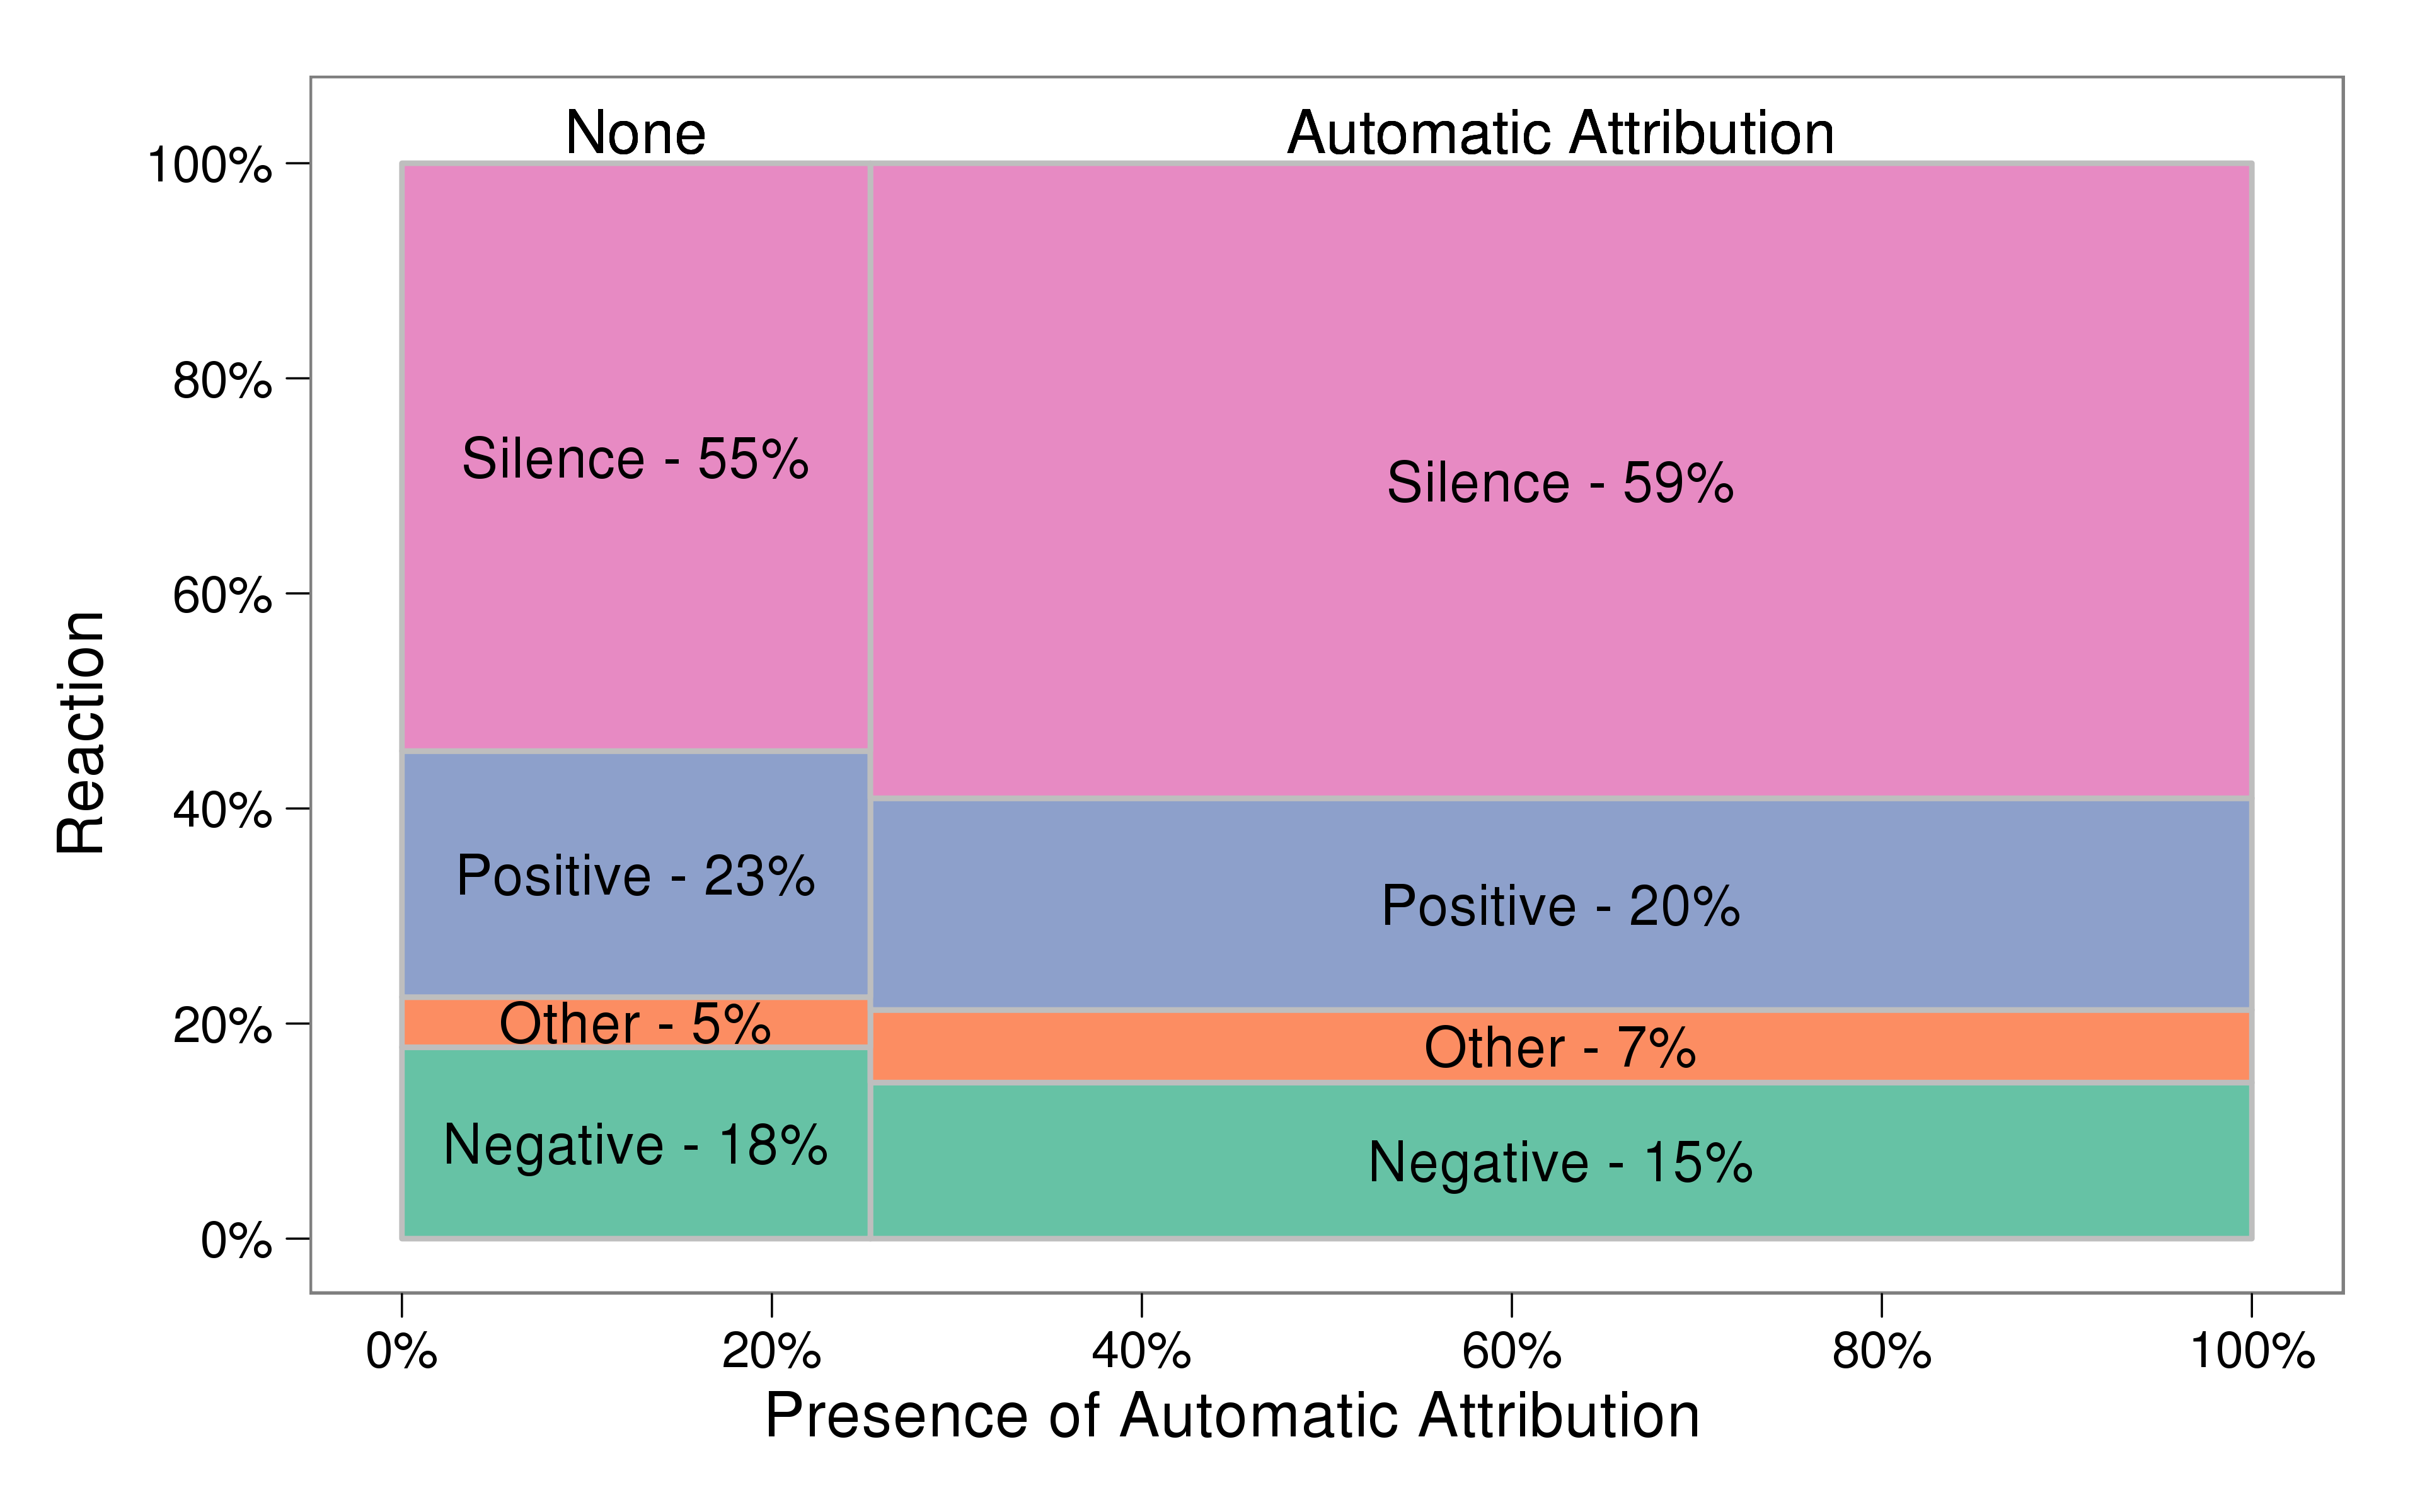
\includegraphics[width=3.3in]{figures/mosaic_automatic_attribution.png}
\caption{Mosaic plot showing the distribution of reactions of original
  creators who had viewed remixes of their project during the six week
  periods before and after the introduction of automatic
  attribution. The proportion of response types is shown along the
  y-axis. The proportion of projects viewed with, and without,
  automatic attribution is shown along the x-axis. ($n=932$)}
\label{fig:mosauto}
\end{center}
\end{figure}

To test the effectiveness of automatic attribution, we consider the
effect of the design intervention described in the previous section.
The design change took place six weeks after the public launch of the
Scratch community and at the precise midpoint in our data collection
window. The intervention affected all projects hosted on the Scratch
online community including projects shared before the automatic
attribution functionality was activated. As a result, we classify
originators' reactions as occurring outside a technological regime of
automatic attribution when a project was both uploaded and viewed by a
project's originator before automatic attribution functionality was
activated.

A comparison of the distribution of coded comments between positive,
neutral, negative, and silent in the periods before and after the
intervention suggests that the introduction of automatic attribution
had little effect on the distribution of reaction types (See Figure
\ref{fig:mosauto}). Although the period after the intervention saw a
larger proportion of users remaining silent and a smaller proportion
of both positive and negative comments, $\chi^2$ tests suggest that
there is no statistically significant difference in originator
reactions between remixes viewed before or after the introduction of
automatic attribution ($\chi^2 = 3.94; df=3; p=0.27$). As a result, we
cannot conclude that the there is any relationship between the
presence, or absence, of an automatic attribution system in Scratch
and the distribution of different types of reactions.

These results suggest that automatic attribution systems may have
limited effectiveness in communities like Scratch. Of course, our
analysis is not without important limitations. For example, the
existence of an automatic attribution regime may also affect the
behavior of users preparing remixes. A remixer might avoid making
perfect copies of projects if they know that their copies will be
attributed and are more likely to be discovered.

\subsection{Study 1b: Manual Crediting}

While the introduction of an automatic attribution feature to Scratch
appears to have had a limited effect on originators responses to
remixes of their projects, the presence or absence of credit was a
recurring theme in discussions on Scratch online forums -- as shown in
the quotes in the previous section -- and in many of the coded
reactions from the periods both before and after the introduction of
automatic attribution. Indeed, in project descriptions or notes from
the periods both before and after the change, remixers frequently
``manually'' gave credit to the originators of their
work. Even after remixes were automatically attributed to originators,
remixers who did not also give credit manually -- essentially
producing information redundant to what was already being displayed by
the system -- were criticized.

For example, after the introduction of automatic attribution
functionality, a user left the following comment on a remix of their
project:

\begin{quote}
  Bryan, you need to give me Pumaboy credit for this wonderful game
  that I mostly pretty much kinda totally made this whole entire game
  ... and that you need to give me some credit for it
\end{quote}

For this user, automatic attribution by the system did not represent a
sufficient or valid form of credit-giving. In the following study, we
test for this effect of ``manual'' credit-giving by remixers on coded
response types using a method that parallels the analysis in Study 1a
and that uses the same dataset.

Manual crediting can happen in multiple ways.  Exploratory coding of
133 randomly selected projects showed that 35 (36\%) of each remix pair gave
credit.  Of these 35 projects, 34 gave credit in the project
description field while 1 project only gave credit in a ``credits''
screen inside the game. As a result, the authors of this study split
the sample of projects used in the Study 1a and coded each of of the
user-created descriptions for the presence or absence of explicit or
manual credit-giving.

To first establish that we are examining distinct behaviors, we
attempted to establish that automatic and manual attribution do not
act as substitutes for each other. As suggested by our qualitative
findings and our results in Study 1a, we found little difference in
the rate of explicit credit giving between projects created in the
presence or absence of automatic attribution. Overall, 276 (about
30\%) of the 932 projects in our sample offered explicit credit in the
description field of the project. Manual crediting-giving was a
widespread practice both before automatic attribution, when 31\% of
projects in our sample offered explicit credit, and after, when 27\%
did so.  The difference between these two periods was not
statistically significant ($\chi^2=1.41; df=1; p=0.24$). Previous work
studying \emph{Jumpcut}, a video remixing website, supports the idea
that automatic and manual credit giving are not interchangable
phenomena.  One Jumpcut user with permission to creative derivative
works commented that they, ``still feel a moral obligation to people
as creators who have a moral right to be attributed (and notified)
despite the physical design which accomplishes this automatically''
\cite{diakopoulos_evolution_2007}.

\begin{figure}
\begin{center}
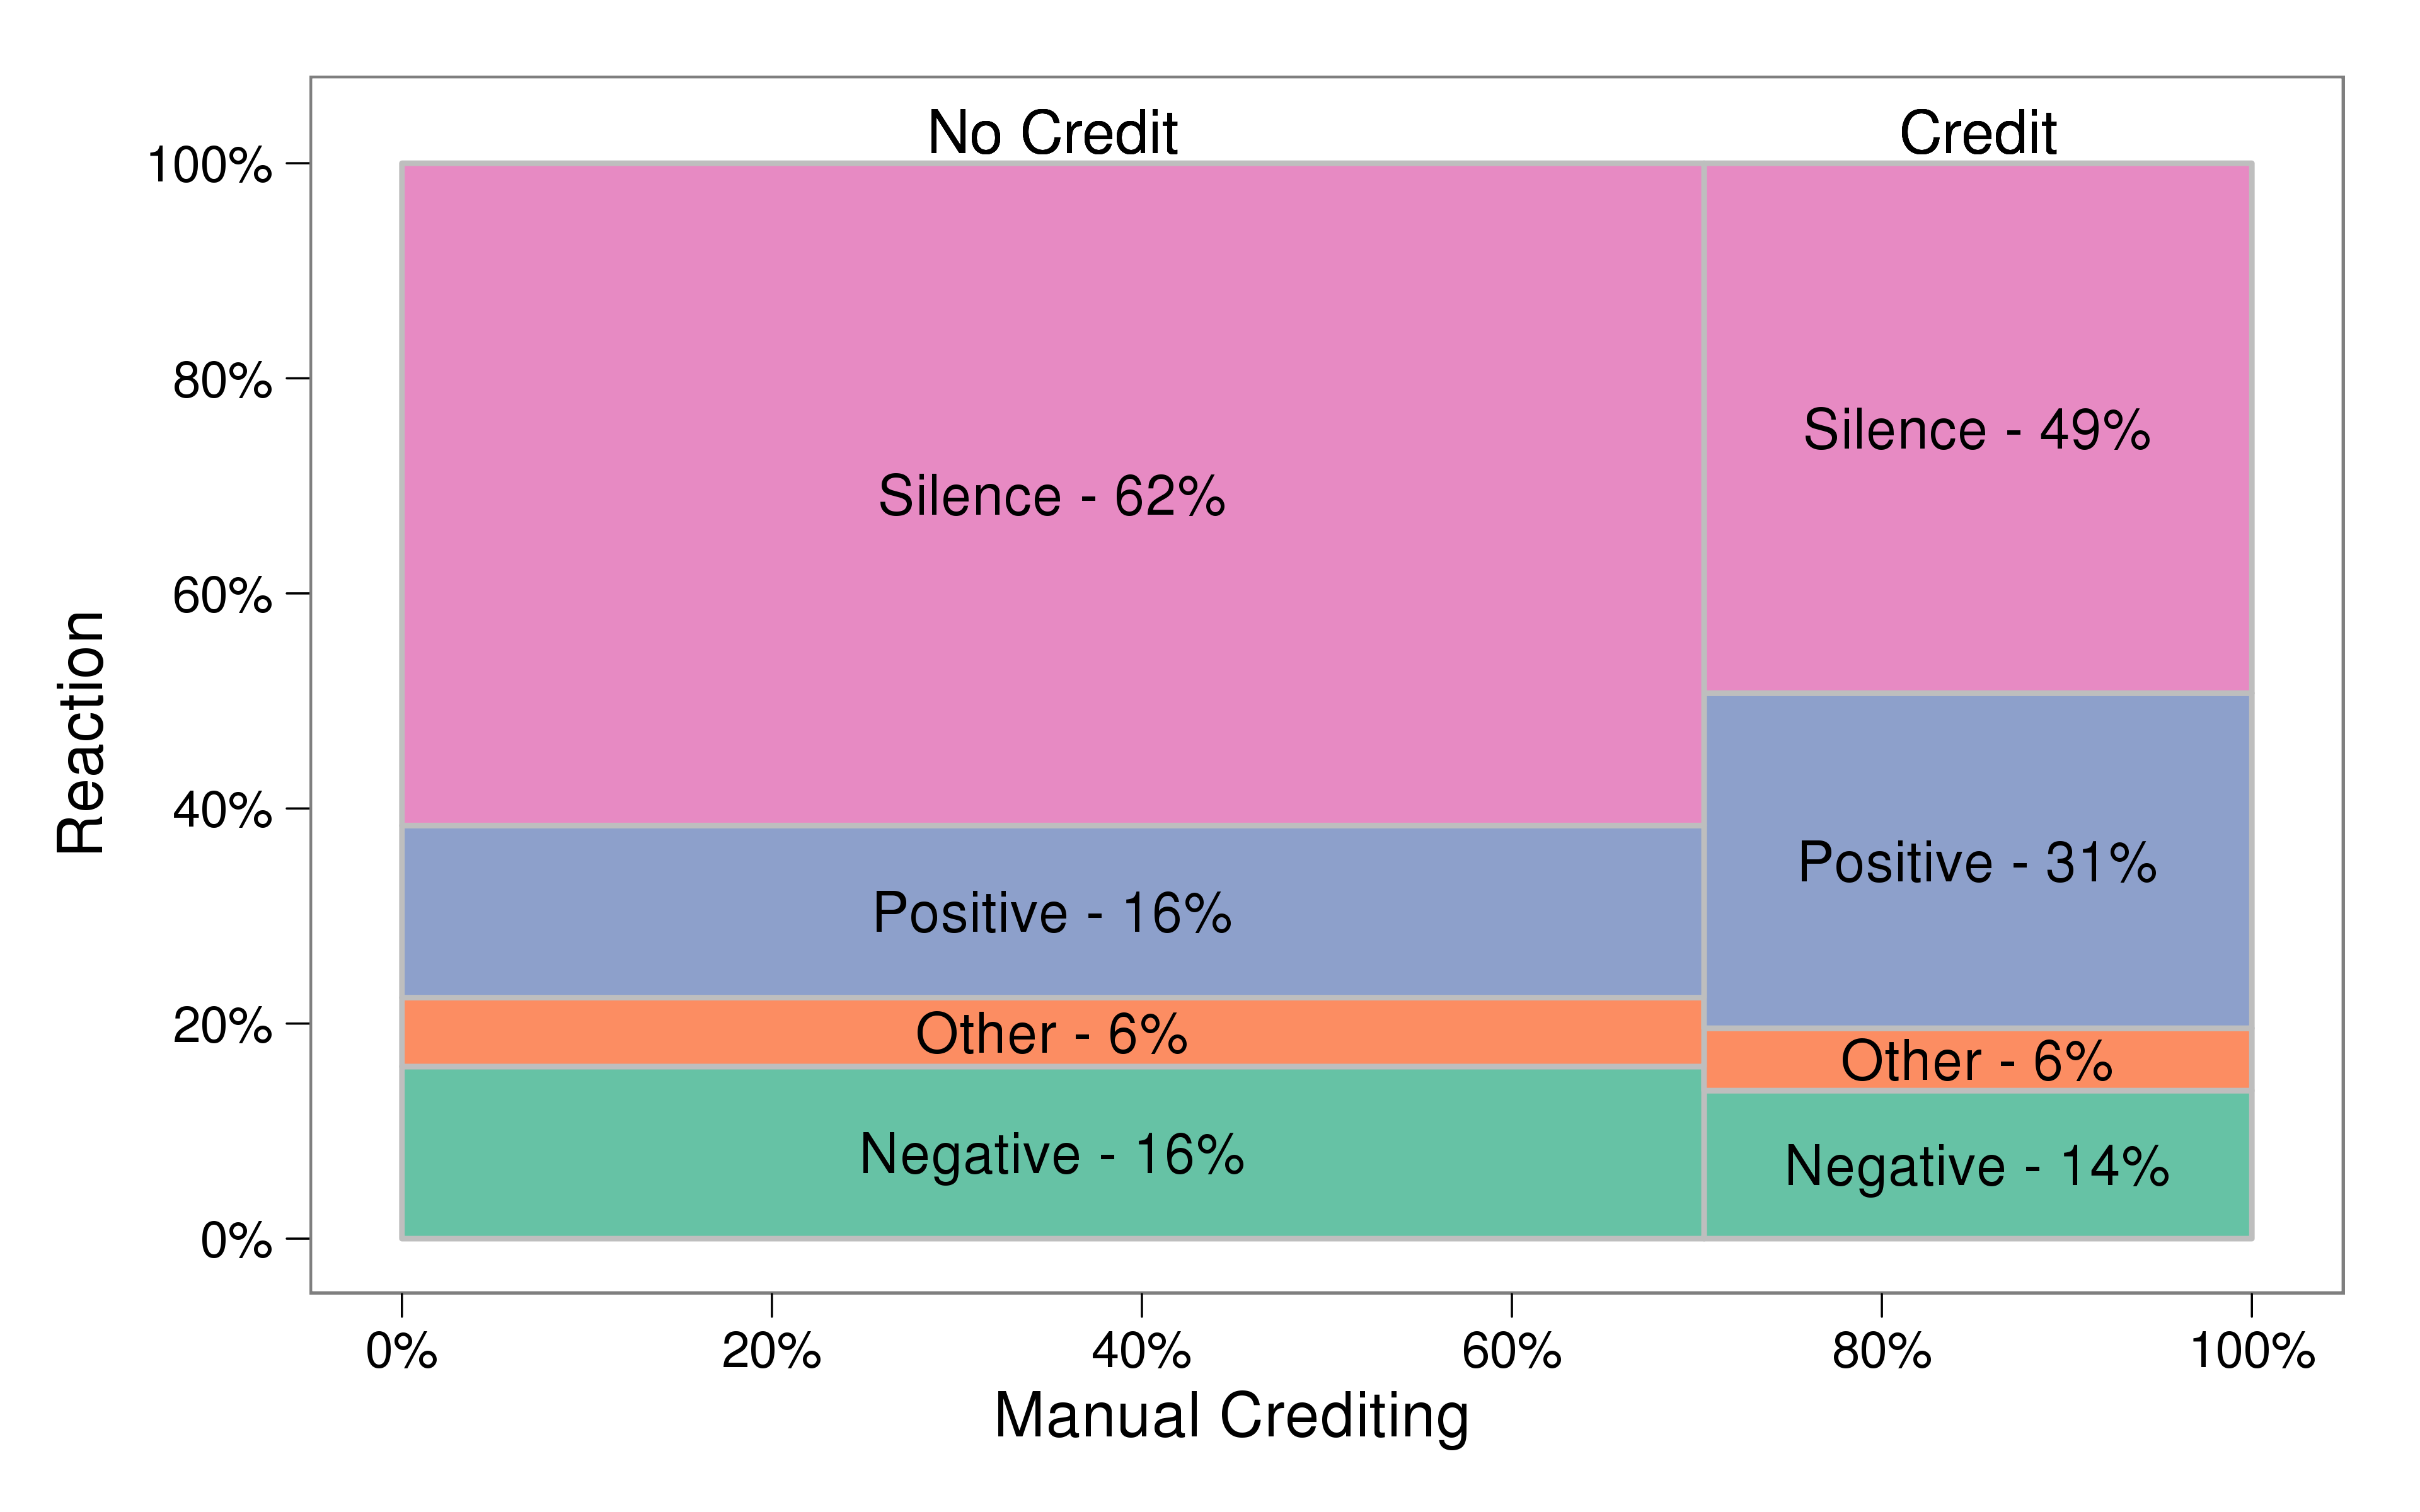
\includegraphics[width=3.3in]{figures/mosaic_manual_credit.png}
\caption{Mosaic plot showing the distribution of reactions of original
  creators who had viewed remixes of their project and indicating
  whether they left manual credit. The proportion of response types is
  shown along the y-axis. The proportion of projects including and
  omitting manual credit is shown along the x-axis. ($n=932$)}
\label{fig:moscredit}
\end{center}
\end{figure}

We measured effectiveness of manual credit giving using a parallel
analysis to Study 1a. As in Study 1a, we compared the distribution of
originator reactions in the presence, and absence, of manual
credit-giving by remixers. We found that negative reactions are less
common in the presence of manual credit but that this difference is
very small (from 16\% without manual credit to 14\% with it). However,
we see that the proportion of users who react positively almost
doubles in the presence of credit-giving (from 16\% with no crediting
to 31\% in its presence). A graph of these results are shown
in Figure \ref{fig:moscredit}. Tests show that we can confidently
reject the null hypothesis that these differences in the distribution
of reactions are due to random variation ($\chi^2 = 27.60; df=3;
p<0.001$).

Also important to note is a difference in the number of users who are
silent after viewing a project (62\% in the absence of manual credit
versus 49\% in its presence). This larger proportion of commenting in
general may have an important substantive effect on the discourse and
behavior on the site because silent originators may, for obvious
reasons, have a more limited effect on attitudes toward remixing and
user experience than vocal users do. As a robustness check, we
considered the reaction of only originators who left comments
($n=388$) and found that even with a smaller sample, our result were
stronger. In the restricted sample, 41\% reacted negatively when they
were not given credit.  However, only 27\% did so when they were
credited. Similarly, 42\% of users who left comments on projects that
did not give credit manually left positive messages. Nearly two thirds
of comments (61\%) were positive when credit was given.  These
differences, in the reduced sample that includes only explicit
reactions, were also statistically significantly different ($\chi^2 =
14.09; df=2; p<0.001$). We include the large number of silent
participants because we believe that non-response is an important type
of reaction with real effects on the community. Understanding the
reasons behind non-response and the effect of silence in response to
different types of credit giving remains an opportunity for further
research.

Although not presented here due to limited space, we followed the
general model of previous work using this dataset
\cite{hill_responses_2010} and tested logistic regression models on
dichotomous variables indicating the presence of negative and positive
reactions and found that basic relationships described above were
robust to the introduction of a control for the the intervention, to
an interaction between these two variables, and to controls for the
gender and age of originators and to the antecedent project's
complexity. Both before or after the intervention, manual crediting
resulted in more positive comments by the originators of remixed
projects. Of course, the results presented here are uncontrolled,
bivariate, relationships and we caution that these results, while
provocative, should still be viewed as largely tentative. As we show
in the subsequent qualitative analysis, attribution and credit-giving
are complex social processes. We do not claim that the preceding
analyses capture it fully.


\section{Study 5: Interviews with participants}

In order to explore the reasoning behind young people's remixing
behavior and attitudes toward attribution as we observed it in Study
1, we engaged in a second qualitative study and directly asked kids
what role attribution and credit plays in their moral evaluations of
remixing.

\begin{table*} \begin{tabular}{lccp{4.5in}} \hline
\textbf{Name (pseudonym)} & \textbf{Age} & \textbf{Gender} & \textbf{Relationship to Scratch}\\
\hline
Nicole & 10 & F & She has created with hundreds of Scratch projects, mainly animations and art ones. \\
Kyle & 14 & M & Casual user of Scratch, interested in math/science simulations and video games. \\
Amy & 15 & F & Avid photographer, has never used Scratch. \\
Charles & 9 & M & Active member of a subgroup of Scratch interested in simulation of operating systems.  \\
Ryan & 12 & F & Long-time member of the Scratch community. Creates complex video games. \\
Jon & 9 & M & Casual user of Scratch, collaborates with Scratch friends in person. \\
Jake & 11 & M & Casual user, likes making video games. \\
Cody & 16 & M & Creates hip hop accessories, not active in Scratch. \\
Paul & 9 & M & Creates Scratch projects with a focus on engineering and video games. \\
Jimena & 17 & F & Highly technical teen with programming experience but no experience with Scratch. \\
Madeline & 14 & F & Very popular animator  in the Scratch community. \\
Susie & 10 & F & Has created hundreds of projects including games, animations and art, but preferring art. \\
\hline
\end{tabular} \caption{Table listing details of interviewees used in Study 2. ($n=12$)} \label{tab:ints} \end{table*}

\subsection{Methodology}

We conducted twelve one-hour semi-structured interviews with kids aged
8 to 17 years old. All of the interviewees had 
experience using
computers and had access to the Internet at home. All the interviewees
live in the United States except for one who lives in New Zealand. The
participants were recruited via the Scratch website and during
meet-ups with educators, teachers and young Scratch users. Eight of
the interviews were conducted in person, in the Boston area, and the
rest over the phone or voice over IP.  The interviews were
audio-recorded and transcribed before fully analyzing them. Nine of
the interviewees were members of the Scratch community.  The remaining
three did not use Scratch but were included as a way to check if
people who do not use Scratch have similar views about remixing,
attribution, and credit. We found no substantive difference between
the Scratch users and non-users in their answers to questions related
to the hypothetical automatic and manual mechanism for attribution.

Before each interview, subjects completed a survey that elicited
demographic information and posed questions about their familiarity
with other technologies and which was primarily designed to get a
sense of the interviewees' social and technical background. Interviews
were structured around a protocol that included a set of nine
fictional remixing cases intended to elicit conversations about
remixing.\footnote{Our interview protocol including example cases is
  available at
  http://www.media.mit.edu/~andresmh/chi2011/interview.html.} The
cases were inspired by Sinnreich et al.'s theoretical work and from
three years of experience moderating the Scratch community. They were
designed to present cases where remixing could be controversial but
where there is no clear ``correct'' answer. The goal of the cases was
to offer a concrete, and common, set of dilemmas to stimulate broad
conversations about attitudes toward remixing.

The cases were presented in the form of printed screenshots of
different project pages from the Scratch website (anonymized to avoid
referring to real cases that users might have seen).
The print outs were shown to the interviewees (or
discussed over the phone) while explaining each case.  All the cases
included a remix and its corresponding antecedent project. The cases varied 
in the presence of automatic attribution, manual credit, and
the degree of similarity between the remix and its antecedent. For example, the
first three cases were:

\begin{enumerate}

\item A remix and its antecedent are identical. The project notes only
  describe how to play the video game. The remix shows the automatic
  attribution but no manual credit on the notes.

\item A remix and its antecedent are different (as seen visually and
  in project metadata) but one can clearly see the influence of its
  antecedent project. The project notes of the remix show manual
  credit but no automatic attribution. The interviewee was told to
  imagine the site had a glitch that prevented it from connecting it
  to its antecedent.

\item The same set of remix and antecedent projects as in (2) but this
  time automatic attribution is displayed but manual credit is not.

\end{enumerate}

Each of the interview logs was coded using
inductive codes and grounded theory \cite{charmaz_constructing_2006}.
The coded responses were analyzed based on categories related to how
interviewees answered specific questions about the distinction between
automatic attribution and manual credit.

\subsection{Results}

Confirming the results of Study 1, for users of Scratch, automatic
attribution was generally seen as insincere and insufficient.
Throughout the interviews, we found that for most of the kids, getting
explicit credit from another person was preferred over attribution
given automatically by the system. When asked why, kids often
responded that knowing that another person had cared enough to give
credit was valued more than what the computer system would do on its
own. The fact that it takes some work, albeit minimal, to write an
acknowledgment statement, sends a signal of empathy, authenticity and
good intentions \cite{donath_signals_2008}. Amy articulated this when
explaining why she preferred getting credit from another person:

\begin{quote}
  I would like it even more if the person did it [gave credit] on their own accord,
  because it would mean that [...] they weren't
  trying to copy it, pirate it.
\end{quote}

Similarly, Jon explained, ``No [the ``Based on'' is not enough],
because he [the remixer] didn't put that, it always says that.'' For
Jon, automatic attribution is not authentic because it is always there
and, as a result, it is clear that is not coming from the person doing
the remix.

Most of the interviewees seemed to have a clear notion of what they
think a moral remix should be. For some, it is all about making
something different. Jake for example, defines a ``good'' remix as,
``if it has a bunch of differences then it’s a good remix. If it has
like two, then it’s bad.''  In addition to the differences between the
remix and its antecedent project, for some, manual credit is part of
what makes it moral. Charles said, ``[remixing] is taking somebody
else's project and then changing a lot of it and sharing it and giving
credit.''  Continuing, Charles explained:

\begin{quote}
  If Green had actually said in the project notes, ``This is a remix
  of Red's project, full credit goes to him,'' then I would consider
  it a remix.  But this [pointing at a remix without manual credit] is
  definitely a copy.
\end{quote}

Likewise, Ryan mentions that a fictional remix was, ``perfectly fine
because they gave credit in the project notes.''

Interviewees suggested that manual credit also allows users to be more
expressive. For example, Susie explained that expressiveness is the
reason that she prefers manual credit through the project notes
saying, ``I think the manual one is better because you can say `thank
you' and things like that.  The automatic one just says `it's based
on.''' Susie also notes that for her, the project notes are a space
where a creator can express her wishes in regards to her intellectual
property, independent, and even in contradiction to, the license of
the projects:

\begin{quote}
  If I do a project that has music that I really like, I often
  download the project, take the music.  Unless it says in the project
  notes, ``Do not take the music.''
\end{quote}

For Susie and other users of Scratch, the project notes are a space
for more than just instructions on how to interact with one's project;
they are an expressive space where one can communicate with an
audience without having to encumber the creative piece of work with
it.

Others point at the fact that people do not pay as much attention to
automatic attribution statement as much they do to the manual credit
left in project descriptions. Jake, for example, explains that, while
he agrees there is some usefulness to having both, project notes still
are more important, ``because, you know, sometimes people just like
skim through a project and you don’t see it ‘til the end.''  Jake
continued to say that creators that do not have both should get a
``warning.''

Even though interviewees value manual credit, they still see the
usefulness of the automatic mechanism as some sort of
community-building prosthetic device -- an explanation for the
positive reactions to the feature's initial introduction. For example,
Nicole argues that while manual credit on the notes has more value for
her, the automatic attribution is useful as a backup and because it
provides a link:

\begin{quote}
  Well, I think that they should probably write in the notes that --
  then it should also say ``Based on blank's project,'' just in case
  they forget, and also because it gives a link to the original
  project and it gives a link to the user so you don't have to search
  for it.
\end{quote}

A similar explanation was articulated on a comment exchange on one the
website's galleries. A teenage girl that actively participates in
Scratch explained the pragmatic value of automatic attribution saying,
``the `based on' thingy, it gives a link, and we all luv links, less
typing,'' before reiterating that manual credit is more valuable:

\begin{quote}
  at the beginning i thought that you don't have to give credit when
  the ``based on'' thingy is in there, but i realized a lot of people
  don't look at that, and i noticed people confused the remix with the
  original.
\end{quote}

% for our records http://scratch.mit.edu/galleries/view/91701?comment=1772604
% do not cite to protect privacy

Creating a Scratch project is a complicated task. A project's sources
can be diverse and the creator can easily forget to acknowledge some,
as Paul explains, when asked to choose between a system of manual
credit or automatic attribution:

\begin{quote}
  The thing is, it would be a lot better if they had both. Because,
  sometimes people probably just forget to do that. And then people
  would not know.
\end{quote}

There are also situations where interviewees recognize what Posner
calls the ``awkwardness of acknowledgment,'' that is, situations where
credit is not really needed and it can be an unnecessary burden or go
against the aesthetics of the work \cite{posner_little_2007}. For
example, Paul mentioned that sometimes, there are some projects in
Scratch that are remixed so much -- like the sample projects that come
with Scratch or some ``remix chains''\footnote{Remix chains typically
  start with someone sharing a project inviting others to remix 
  (i.e. ``add your animated avatar to the park.'')} -- where credit is not
necessary:

\begin{quote}
  There's this one called ``perfect platformer base'' which a lot of
  people remix. So I don't think that needs any credit. It's not
  actually a real game. It's all the levels and stuff are just
  demonstrations.
\end{quote}

Since manual crediting has a higher emotional value, some kids
mentioned that conflicts over remixing could be addressed by the
administrators of the site by editing the project of the remix in
question, as a way to enforce credit without transforming it into
attribution. Doing so would make it appear that a remixer had credited
an antecedent when they had not. Susie offers a suggestion along these
lines when asked about how the administrators of the website should
deal with a case of a complaint over a remix that is a parody of
someone else's project. Susie suggested that, ``I might remove the
project but I might not, you know, maybe I would edit the notes to to
give credit.''  Similarly, Charles described his approach for solving
conflicts if he was the administrator of the website suggesting that,
``I probably just would stay out of the argument.  I probably wouldn't
remove it [the remix], I'd just add something in the project notes
[like] `based on Gray's project.'''

This phenomena of giving less value to technologically simplified
social signals is experienced in other social platforms. For example,
Amy expressed how on the social network site Facebook, she loves to
get comments on her photographs but dislikes those who do not leave
comments or opt instead to press the ``I like it'' button:

\begin{quote}
  I love when people comment on my pictures.  Everybody sees them,
  because they tell me they have.  I'm like, ``Oh really?  That's
  great.  Why didn't you comment?'' I don't like it when people just
  ``like it'', because you know they have something to say about it;
  they just don't.  It's like, if they like it, then [they should]
  take the time to say something.
\end{quote}

Although not designed to be a random sample, these interviews support
the proposition that both Scratch participants and other young people
share a set of norms about characteristics that determine what a
``good'' or moral remix is. Among these norms, acknowledging one's
sources seems to play a central role. However, participants also seem
to share the opinion that this norm is not satisfied through an
automated process.  They clearly understand the pragmatic value of
automating acknowledgment-giving, but
they do not see it as a substitute for adherence to the social norm of
credit-giving. They also see it as void of emotion and expressiveness.
For Scratch users, normative constraints are separate from
architectural constraints and one cannot replace the other.
These findings support and enrich the results from our first
study and help us understand better how Scratch participants, and
perhaps kids in general, experience authorship norms and automation in
online spaces.

\section{Conclusions}

Our results from Study 1a called into the question the effectiveness
of automatic attribution functionality in encouraging more positive
user reactions in Scratch. We build on these results in Study 1b to
suggest that manual crediting may do the work that Scratch's designers
had hoped automatic attribution would. Results from the analysis of
user interviews presented in Study 2 help to answer the question of
``why?'' and suggest that users find manual credit to be more
authentic and more meaningful to users because it takes more time and
effort. Usually, UI  improvements are designed to help reduce the time
and effort involved in using a system. But in trying to help users by attributing automatically,
Scratch's designers misunderstood the way that attribution as a social
mechanism worked for Scratch's users. Our fundamental insight is that
while both attribution and credit may be important, they are distinct
concepts and that credit is, socially, worth more. A system can
\emph{attribute} the work of a user but \emph{credit}, which is seen
as much more important by users and which has a greater effect on user
behavior, cannot be done automatically. Computers can
attribute. Crediting, however, takes a human.

As we suggested in our introduction, this fundamental result leads to
two distinct contributions. First, and more specifically, our analysis
offers an improved understanding of the way that attribution and
credit works in user-generated content communities over what has been
available in previous work. Our two studies suggest that scholars are
correct to argue that credit plays an important role in social media
communities and offer empirical confirmation for the important role
that authenticity plays in how users conceptualize credit. In our
in-depth interviews, we explain some of the reasons why this may be
the case. Second, through our evaluation of an unsuccessful
technological design, our work offers a broader, if more preliminary,
contribution in suggesting an important limit of designers' ability to
support community norms in social media systems. As the literature on
design and social media grows, the importance of good support for
communities with healthy norms promoting positive interactions is
likely to increase. In attempting to design for these norms, we
suspect that researchers will increasingly encounter similar
challenges.

We argue that designers should approach interventions iteratively.
This design approach can be understood through the
theoretical lens of the social construction of technology
\cite{pinch_social_1984}: designers can't control technological outcomes which
must be built through a close relationship between designers and users.
Designers must move away from seeing their profession as
providing solutions. They must channel users, work closely with them,
and iterate together, to negotiate and achieve a set of shared goals.

The prevalence of user-generated content sites stresses the importance
of how online social spaces should deal with issues of attribution and
our results are likely to be immediately relevant to 
designers. For example, the Semantic Clipboard is a tool built as a
system of automatic attribution for content reuse
\cite{seneviratne_policy-aware_2009}. Developed by researchers who
found a high degree of Creative Commons license violations around the
re-use of Flickr images, the tool is a Firefox plugin that provides,
``license awareness of Web media,'' and enables people to
automatically, ``copy [media] along with the appropriate license
metadata.'' Our results suggest one way that this approach
may fall short.

However, automatic attribution is not the only way that technologists
can design to acknowledge others' contributions. Indeed, our results
suggest that there may be gains from design changes which encourage
credit-giving without simply automating attribution. For example,
Scratch's designers might present users with a metadata field that
prompts users to credit others and suggests antecedent authors whose
work the system has determined may have played a role. This affordance
might remind users to credit others, and might increase the amount of
crediting, while maintaining a human role in the process and the extra
effort that, our research has suggested, imbues manual credit giving
with its value. We suggest that in other social media communities,
similar affordances that help prompt or remind users to do things that
a system might do automatically represent a class of increasingly
important design patterns and a template for successful design
interventions in support of community norms.

% TODO Importance of findings to the design of online communities by
% Krout's MovieLens % should this be in Intro?




\section{Study 7: Plasticity of Virtue.}
For the past five months, I have been running an experiment aimed at ascertaining how people's attitudes toward remixing could be changed through a design intervention.
The study consists of sending notification messages that try to appeal to various motivations for cooperating in the Scratch online community. 
As mentioned before, a contentious issue in the Scratch community has been the acceptance of remixing by those whose projects are remixed. 
People only learn about remixes of their projects by browsing their project pages and looking at the list of derivative works. 
The notification page is the principal form of communication between the system and the users.
The experiment consists of informing people when one of their projects gets remixed.
This experiment provides an opportunity to test: 1) the comparative effectiveness of various ways of communicating the same event and 2) the permanency of the behavioral change, if any. 

The experiment consists of two phases.
The first is the notification period. 
When someone's project gets remixed, the system automatically assigns the creator of that project to one of the treatment conditions. 
From then on, the person receives messages whenever someone remixes his or her project. The message depends on the treatment category.
For example some messages are neutral (for example, ``Your project FooBar was remixed. Check out the remix.''); 
others are positive (for example,``Congratulations! Your project FooBar was remixed. Check out the remix .'');
others try to elicit generosity (for example, ``Your project FooBar has been remixed. Sharing your work is a generous thing to do and a great thing for the Scratch community! Check out the remix.'').
Other messages try to elicit conformity, reputation building and fairness.
Finally, a control category is added where no notification is sent.

The second phase of the experiment is sending no notifications. In this phase of the experiment, the notifications stop and people's reactions continue to be logged.

After a few weeks we look at the results of pre- and post-phase one, to analyze the effectiveness of each treatment by measuring the number of positive and negative reactions that originators leave on the remixes. 
Additionally, I analyze the pre- and post-phase two, to see how malleable the behavior is.

\section{Study 8: Featuring Top Remixes.}
The home page of the Scratch website now has a section called ``What the Community is Remixing''  that features the three top remixed projects in the past two weeks.
This section did not exist when the website was first unveiled.
In fact, this section was added as measure to counter the backlash against remixing by showing that getting one's project remixed could increase social status in the community (being on the front page is an important reputation-building mechanism).
This study aims at assessing whether a design intervention aimed at increasing the acceptance of remixing had a ``crowding out'' effect by decreasing the quality or effort people put into making their remixes.
I have devised metrics to operationalize the complexity and effort a creator puts into creating his or her project. These metrics are based on the number of sprites, scripts, blocks, diversity of blocks and time it took from the first save to the hard disk until it gets shared on the website.



